%% Copernicus Publications Manuscript Preparation Template for LaTeX Submissions
%% ---------------------------------
%% This template should be used for copernicus.cls
%% The class file and some style files are bundled in the Copernicus Latex Package, which can be downloaded from the different journal webpages.
%% For further assistance please contact Copernicus Publications at: production@copernicus.org
%% https://publications.copernicus.org/for_authors/manuscript_preparation.html


%% Please use the following documentclass and journal abbreviations for discussion papers and final revised papers.

%% 2-column papers and discussion papers
%\documentclass[journal abbreviation, manuscript]{copernicus}
\documentclass[se, manuscript]{copernicus}



%% Journal abbreviations (please use the same for discussion papers and final revised papers)


% Advances in Geosciences (adgeo)
% Advances in Radio Science (ars)
% Advances in Science and Research (asr)
% Advances in Statistical Climatology, Meteorology and Oceanography (ascmo)
% Annales Geophysicae (angeo)
% Archives Animal Breeding (aab)
% ASTRA Proceedings (ap)
% Atmospheric Chemistry and Physics (acp)
% Atmospheric Measurement Techniques (amt)
% Biogeosciences (bg)
% Climate of the Past (cp)
% DEUQUA Special Publications (deuquasp)
% Drinking Water Engineering and Science (dwes)
% Earth Surface Dynamics (esurf)
% Earth System Dynamics (esd)
% Earth System Science Data (essd)
% E&G Quaternary Science Journal (egqsj)
% European Journal of Mineralogy (ejm)
% Fossil Record (fr)
% Geochronology (gchron)
% Geographica Helvetica (gh)
% Geoscience Communication (gc)
% Geoscientific Instrumentation, Methods and Data Systems (gi)
% Geoscientific Model Development (gmd)
% History of Geo- and Space Sciences (hgss)
% Hydrology and Earth System Sciences (hess)
% Journal of Micropalaeontology (jm)
% Journal of Sensors and Sensor Systems (jsss)
% Magnetic Resonance (mr)
% Mechanical Sciences (ms)
% Natural Hazards and Earth System Sciences (nhess)
% Nonlinear Processes in Geophysics (npg)
% Ocean Science (os)
% Primate Biology (pb)
% Proceedings of the International Association of Hydrological Sciences (piahs)
% Scientific Drilling (sd)
% SOIL (soil)
% Solid Earth (se)
% The Cryosphere (tc)
% Weather and Climate Dynamics (wcd)
% Web Ecology (we)
% Wind Energy Science (wes)


%% \usepackage commands included in the copernicus.cls:
%\usepackage[german, english]{babel}
%\usepackage{tabularx}
%\usepackage{cancel}
%\usepackage{multirow}
%\usepackage{supertabular}
%\usepackage{algorithmic}
%\usepackage{algorithm}
%\usepackage{amsthm}
%\usepackage{float}
%\usepackage{subfig}
%\usepackage{rotating}


\begin{document}

\title{Estimating ocean tide loading displacements with GPS and GLONASS}


% \Author[affil]{given_name}{surname}

\Author[1]{Bogdan}{Matviichuk}
\Author[1]{Matt}{King}
\Author[1]{Christopher}{Watson}

\affil[1]{School of Technology, Environments and Design, University of Tasmania, Hobart, 7001, Australia}
%\affil[]{ADDRESS}

%% The [] brackets identify the author with the corresponding affiliation. 1, 2, 3, etc. should be inserted.

%% If an author is deceased, please mark the respective author name(s) with a dagger, e.g. "\Author[2,$\dag$]{Anton}{Aman}", and add a further "\affil[$\dag$]{deceased, 1 July 2019}".

%% If authors contributed equally, please mark the respective author names with an asterisk, e.g. "\Author[2,*]{Anton}{Aman}" and "\Author[3,*]{Bradley}{Bman}" and add a further affiliation: "\affil[*]{These authors contributed equally to this work.}".


\correspondence{Bogdan Matviichuk (bogdan.matviichuk@utas.edu.au)}

\runningtitle{Estimating ocean tide loading displacements with GPS and GLONASS}

\runningauthor{B. Matviichuk et al.}



\received{}
\pubdiscuss{} %% only important for two-stage journals
\revised{}
\accepted{}
\published{}

%% These dates will be inserted by Copernicus Publications during the typesetting process.


\firstpage{1}

\maketitle



\begin{abstract}
Ground displacements due to ocean tide loading have previously been successfully observed using GPS data, and such estimates for the principal lunar $M_2$ constituent have been used to infer the rheology and structure of the asthenosphere. The GPS orbital repeat period is close to that of several other major tidal constituents ($K_1$,$K_2$,$S_2$) thus GPS-estimates of ground displacement at these frequencies are subject to GPS systematic errors. We assess the addition of GLONASS to increase the accuracy and reliability of eight major ocean tide loading constituents: four semi-diurnal ($M_2$, $S_2$, $N_2$, $K_2$) and four diurnal constituents ($K_1$, $O_1$, $P_1$, $Q_1$). We revisit a previous GPS study, focusing on 21 sites in the UK and western Europe, expanding it with an assessment of GLONASS and GPS+GLONASS estimates. In the region, both GPS and GLONASS data are abundant since 2010.0. We therefore focus on the period 2010.0-2014.0 which is considered long enough to reliably estimate the major constituents. Data were processed with a kinematic PPP strategy to produce site coordinate time series for each of 3 different modes: GPS, GLONASS and GPS+GLONASS. The GPS solution with ambiguities resolved was used as a baseline for performance assessment of the additional modes. GPS+GLONASS shows very close agreement with ambiguity resolved GPS for lunar constituents ($M_2$, $N_2$, $O_1$, $Q_1$) but with substantial differences for solar-related constituents ($S_2$, $K_2$, $K_1$, $P_1$). While no single constellation mode performs best for all constituents and components, we propose to use a combination of constellation modes to recover tidal parameters: GPS+GLONASS for most constituents except for $K_2$ and $K_1$ where GLONASS (north and up) and GPS with ambiguities resolved (east), perform best.
\end{abstract}


%\copyrightstatement{TEXT}


\introduction %% \introduction[modified heading if necessary]
Earth’s gravitational interactions with the Sun and the Moon generate solid Earth and ocean tides. These tides produce periodic variations in both the gravity field and Earth’s surface displacement. Additionally, the ocean tides produce a secondary deformational effect due to associated periodic water mass redistribution, known as Ocean Tide Loading (OTL) \citep[e.g.,][]{Agnew2015,Jentzsch1997,Baker1984}. 
OTL is observable in surface displacements (and their spatial gradients, i.e. tilt and strain) and gravity. Displacement and gravity attenuate approximately as the inverse of the distance from the point load while gradients have this relation but with distance squared \citep{Baker1984}. Thus, OTL displacement and gravity changes show greater sensitivity to regional solid Earth structure in comparison to tilt or strain observations \citep{Martens2016}, making this an observation of interest for studying solid Earth rheology.

Global Navigation Satellite Systems (GNSS) are particularly convenient for measuring OTL displacements due to the widescale deployment of dense instrument arrays. Data from continuous GNSS stations have been shown to provide estimates of OTL with sub-millimetre precision using two main approaches as described by \cite{Penna2015}: the harmonic parameter estimation approach – OTL displacement parameters are solved for within a static GNSS solution \citep[e.g.,][]{Schenewerk2001,Allinson2004,King2005,Thomas2006,Yuan2012,Yuan2013}; and the kinematic approach – OTL constituents are predominantly estimated from high-rate kinematic GNSS-derived time series \citep[e.g.,][]{Khan2001,King2003,King2006,Penna2015,Martens2016,Wang2019}. In this paper, we follow the kinematic approach.

To date, GNSS-derived OTL displacements have been estimated using predominantly the US Global Positioning System (GPS). GPS-derived measurements of Earth-surface displacement at tidal periods have been successfully used to observe OTL displacement and validate ocean tide models \citep{Urschl2005,King2005}. The residual displacement between observed and predicted OTL has been related to deficiencies in ocean tide models, reference-frame inconsistencies, Earth model inaccuracies, the unmodelled constituents’ dissipation effect and systematic errors in GPS \citep[e.g.,][]{Thomas2006,Ito2011,Yuan2013,Bos2015}.

Recent studies have made use of GPS-derived OTL to study dissipation or anelastic dispersion effects in the shallow asthenosphere at the $M_2$ frequency \citep[e.g.][]{Bos2015}. This type of investigation has not been easily done previously due to various limiting factors such as the accuracy of ocean tide models and the quality and availability of GNSS observations. Recently, however, these have improved dramatically with altimeter-constrained ocean tide models \citep{Stammer2014} and expanding GNSS networks. These have allowed for the demonstration of limitations in the global seismic Preliminary Reference Earth Model (PREM) \citep{Dziewonski1981} with GPS observations in the western United States \citep{Ito2011,Yuan2012}, western Europe \citep{Bos2015}, South America \citep{Martens2016}, Eastern China Sea region \citep{Wang2019} and globally \citep{Yuan2013}. These limitations are associated partially with the incompatibility of the elastic parameters within the seismic (1 s period) and the tidal frequency bands and the anelasticity of the upper layers of the Earth, particularly the asthenosphere. Considering the major lunar tidal constituent, M2, \cite{Bos2015} and, later, \cite{Wang2019} concluded that GPS-derived OTL displacement estimates were different to modeled displacements due to asthenospheric anelasticity. \cite{Lau2017} used results from the global study of \cite{Yuan2013} to constrain Earth’s deep-mantle buoyancy.

Previous studies have highlighted an apparently large error in solar-related constituents estimated from GPS, in particular $K_2$ and $K_1$. This is in part due to their closeness to the GPS orbital ($K_2$) and constellation ($K_1$) repeat periods, which strongly aliases with orbital errors. The closeness to the GPS constellation repeat period may induce interference from other signals such as site multipath which will repeat with this same characteristic period \citep{Schenewerk2001,Urschl2005,Thomas2006}. Additionally, the $P_1$ constituent has a period close to that of 24 hours which is the timespan used for the IGS-standard orbit and clock products \citep{Griffiths2009}, and hence may be contaminated by day-to-day discontinuities present in the products \citep{Ito2011}.

\cite{Urschl2005} proposed that the addition of GLONASS (GLObal NAvigation Satellite System), a GNSS developed and maintained by Russia (USSR before 1991), could improve the extraction of $K_2$ and $K_1$ constituents as the orbit period of the GLONASS satellites ($\sim$11 h 15 min 44 sec) and constellation repeat period ($\sim$8 days) are well separated from major tidal frequencies. However, for many years GLONASS suffered from an unstable satellite constellation and very sparse network of continuous observing stations. This has been progressively addressed over the last decade to the point where many national networks now include a high density of GLONASS (and other GNSS) receivers.

We seek to improve estimates of OTL displacement from continuous GNSS data, especially for constituents that are subject to systematic error in GPS-only solutions (e.g. $S_2$, $K_2$, $K_1$, $P_1$) as found in previous studies \citep{Allinson2004,King2006,Yuan2012}. We do this by using both GLONASS and GPS data to estimate amplitudes and phases for the eight major OTL constituents ($M_2$, $S_2$, $N_2$, $K_2$, $K_1$, $O_1$, $P_1$, $Q_1$). Our work focuses particularly on understanding the sensitivity of estimates to different processing choices.

\section{Dataset}
The sites used in our study are shown in Figure 1, with a focus on south-west England where a large $M_2$ OTL signal is present. Of the 21 stations, 14 stations are in south-west England: covering both sides of Bristol channel (ANLX, SWAS, CARI, CAMO, PADT, APPL, TAUT) and northern coast of English Channel up to Herstmonceux (PMTH, PRAE, EXMO, PBIL, POOL, CHIO, SANO, HERT) with one site (BRST) in the south. Two sites are in northern England (WEAR, LOFT), two in Scotland (LERI, BRAE) with one site in central Europe (ZIM2). All sites are equipped with GPS+GLONASS receivers. Note that sites CAMO, LERI and ZIM2 sites replace CAMB, LERW and ZIMM respectively, which were used by \cite{Penna2015}, to allow for use of GLONASS data recorded at the former set of sites.

Aside from the addition of GLONASS data, an important difference to the study of \cite{Penna2015} is the shift in time period from 2007.0–2013.0 to 2010.0–2014.0. This shift provides sufficient GLONASS data following the upgrade of many receivers to track GLONASS from 2009 that followed the restoration of GLONASS constellation finished (24 SVs) in March 2010. Despite this covering a shorter time span, the length of continuous observations within each site (minimum availability of 0.95 through dataset) exceeds the recommended $\sim$1000 days of continuous observations (4 years with 0.7 availability) \citep{Penna2015}. While the selected time period is fully covered by a complete set of reprocessed orbit and clock products.

The chosen sites experience a range of $M_2$ up OTL amplitudes ranging from > 30 mm (ANLX, APPL, BRST, CAMO, PADT, PRAE), 15-30 mm (CARI, EXMO, LOFT, PBIL, SWAS, TAUT) and < 15 mm (BRAE, CHIO, LERI, POOL, SANO, WEAR, ZIM2).

%figure 1
\begin{figure}[t]
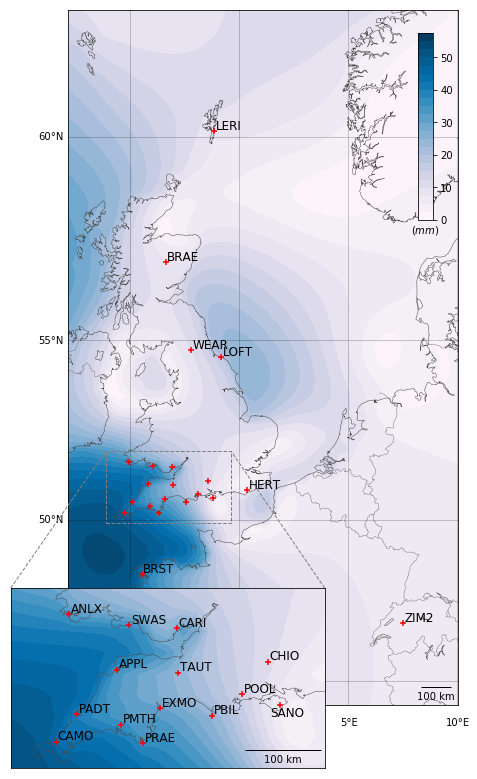
\includegraphics[width=8.3cm]{fig01_updated.png}
\caption{Map of the study area with GNSS site codes and $M_2$ up displacement amplitude in the background (TPXO7.2 ocean tide model and spherically symmetric earth with PREM structure).}
\end{figure}

\section{GNSS data processing strategy}

The processing strategy was largely based on the GPS-only kinematic Precise Point Positioning (PPP) approach \citep{Zumberge1997} %do we really need to cite Zumberge?
as per \cite{Penna2015}, but with modifications in terms of the software and to permit the inclusion of GLONASS data. We address PPP in three different modes here: GPS, GLONASS and combined GPS+GLONASS. In particular, we use NASA JPL’s GipsyX (v. 1.3), which is a substantial rewrite of the now legacy GIPSY-OASIS code to allow for, amongst other things, multi-GNSS analysis. \cite{Penna2015} used GIPSY-OASIS v6.1.2.
We adopted a PPP solution approach and estimated station positions every 5 minutes with a random walk model introducing estimated optimum between-epoch constraints on coordinate evolution. We used the VMF1 gridded troposphere mapping function, based on the European Centre for Medium-Range Weather Forecasts (ECMWF) numerical weather model \citep{Boehm2006}. Additionally, ECMWF values for the hydrostatic zenith delay and wet zenith delay were used as a priori values for stochastic estimation of the wet zenith delay as a random walk process with optimum process noise values (Sect. 4) and tropospheric gradients were estimated as a random walk process \citep{Bar-Sever1998}, with process noise at 0.005 mm/sqrt(s). An elevation cut-off angle of seven degrees was applied together with observation weights a function of the square-root of the sine of the satellite elevation angle.

Earth body-tide (EBT) and pole tides were modelled according to IERS Conventions \citep{IERS2010}. The OTL displacement within each processing run was modelled with the FES2004 tidal atlas \citep{Lyard2006} and elastic Green’s functions based on the Gutenberg-Bullen Earth model \citep{Farrell1972} (FES2004\_GBe), with centre-of-mass correction applied depending on the adopted orbit products. All OTL values used in the pulication were generated using CARGA software at the free ocean tide loading provider (http://holt.oso.chalmers.se/loading) \citep{bos_baker_2005}.

PPP requires pre-computed precise satellite orbit and clock products for each constellation processed which should be solved for simultaneously within a single product's solution. Unfortunately, JPL’s native clock and orbit products are not yet available for non-GPS constellations hence we adopted products from two International GNSS Service (IGS) \citep{Johnston2017} Analysis Centres (ACs): the European Space Agency (ESA) and Centre for Orbit Determination in Europe (CODE). The ESA combined GPS+GLONASS products from the IGS second reprocessing campaign (repro2) were used \citep{Griffiths2019} while CODE’s more recent REPRO\_2015 campaign \citep{repro2015} had to be used as CODE’s repro2 are lacking separate 5 min GLONASS clocks.

All three products consist of satellite orbits and clocks, sampled at 15 and 5 minutes respectively, that were held fixed during our processing. The benefit of using JPL’s native products, even though solely GPS, is the ability to do PPP processing with integer ambiguity resolution (AR). PPP AR in GIPSY-OASIS/GipsyX software can be performed by using wide lane and phase bias tables which are part of JPL’s native products \citep{Bertiger2010}. To provide comparison with previous studies, GPS was processed with JPL’s native orbit and clock products from the repro2 campaign (JPL’s internal name is repro2.1) with AR.

The CODE and ESA clock and orbit products were generated in different ways. CODE’s REPRO\_2015 orbit positions were computed using a 3-day data arc, while ESA used a 24-h data arc \citep{Griffiths2019}. Both ACs provided orbits in a terrestrial reference frame, namely IGS08 and IGb08, respectively, that are corrected for the centre of mass (geocentre) motion associated with OTL (FES2004 centre of mass correction) and are in the CE frame, following \cite{fu_effect_2012}. Alternatively, JPL products were generated from a 30-h data arc, and were computed with stations in a near-instantaneous frame realisation hence the orbits are in the CM frame (we note that the JPL products distributed by the IGS are, by contrast, in CE). Considering the above, the modelled OTL values for JPL’s native products solutions were corrected for the effect of geocentre motion while ESA/CODE products do not require this correction \citep{Kouba2009}.

It has been suggested that orbit arc length for a given product could potentially impact the estimated OTL displacements. In particular, \cite{Ito2011} suggest that a 24-h data arc length (as per ESA products) may affect the $P_1$ constituent due to similarity of the periods. This is in addition to day-boundary edge effects given analysis of data in 24-h batches. We mitigate these effects to some extent by processing the ground stations in 30-h batches (allowing 3-h either side of the nominal 24-h day boundary).

We post-processed the estimated coordinate time series as per \cite{Penna2015}: the resulting 5-min sampled solutions were clipped to the respective 24-h window and merged together. Outliers were filtered from the raw 4-yr timeseries  using two consecutive outlier-detection strategies: rejecting epochs with extreme clock bias values ($>3 \times 10^{3}$ m) or where the XYZ $\sigma$ was over 0.1 m; and then rejecting epochs with residuals to a linear trend larger than three standard deviations per coordinate component. The XYZ timeseries were converted to a local east-north-up coordinate frame, detrended and resampled to 30-min sampling rate via a simple 7-point window average (7 samples -> 1 sample). 30-min averaging reduces high frequency noise (unrelated to OTL) as well as the computational burden of further harmonic analysis.

Finally, OTL displacements modelled in GipsyX were added back using HARDISP \citep{IERS2010}. HARDISP uses spline interpolation of the tidal admittance of 11 major constituents to infer values of 342 tidal constituents and generate a time series of tidal displacements. This approach almost eliminates the effect of companion constituents \citep{Foreman1989} as they are modelled during the processing stage; small errors in the modelled major OTL constituents will propagate into negligible errors in modeled companion tides. Thus, the analysed harmonic displacement parameters represent true displacement plus indiscernible companion constituent error, far below the measurement error. The findings in our paper are in the context of GipsyX software and solutions derived using other software may produce different results especially if the underlying model choices differ.

The harmonic analysis of the reconstructed OTL signal was performed using the Eterna software v.3.30 \citep{Wenzel1996}, resulting in amplitudes and local tidal potential phase lags negative which are suitable for solid Earth tide studies. OTL phase-lag, however, is defined with respect to the Greenwich meridian and phase lags are positive. Transforming to Greenwich-relative lags was done according to \cite{Boy2003} and \cite{Bos2000}.

We then computed the vector difference between the reconstructed observed OTL and that predicted by the model, following the notation of \cite{Yuan2013}:

\begin{equation}
Z_{res} = Z_{obs}- Z_{th}
\end{equation}

In Eq. 1 we assume body tide errors to be negligible, thus $Z_{obs}$ is simply an observed OTL and $Z_{th}$ is a theoretical OTL while $Z_{res}$, residual OTL, is their vector difference. $Z_{res}$ presented in this paper is, if not otherwise specified, relative to the theoretical OTL values computed using the FES2014b ocean tide atlas, a successor of FES2012 used in \cite{Bos2015}, and a Green’s function based on the STW105 Earth model additionally corrected for dissipation at the $M_2$ frequency which we call STW105d (FES2014b\_STW105d). We utilize box-and-whisker plots to demonstrate the distribution of the estimates with the box and whiskers defined as the inter-quartile range (IQR) and an additional \pm 1.5\times \text{IQR}, respectively, with median as a horizontal line.

\section{Process noise optimization}
Process noise settings within GipsyX need to be chosen to ensure optimal separation of site displacement, tropospheric zenith delays, noise etc. For example, a tight coordinate process noise value, even the default value of 0.57 mm/sqrt(s), tend to clip OTL amplitudes, especially in coastal sites. \cite{Penna2015} developed a method of tuning process noise values for GPS PPP, which we expanded to accommodate the additional major diurnal/semidiurnal constituents considered here, as well as the use of GPS and GLONASS data.

To do this, we used the CAMO site, the successor of CAMB used by \cite{Penna2015} and tested a range of coordinate and Zenith Wet Delay (ZWD) process noise settings exactly as described by \cite{Penna2015}. These tests focus on a range of metrics, namely the standard deviation of the height time series (shown as “Ht std/3”, as divided by 3), the standard deviation of kinematic ZWD normalized by ZWD values from a static solution (“ZWDstatic”), root mean square of the carrier phase residuals (“RMSres”), $M_2$ residual OTL magnitude, $\|Z_{res}\|$, and $\|Z_{res}\|$ of a synthetic $\sim$13.96 h signal and its controlled, known input (designated “synth err”). We discuss the results of the "synth\_err" tests in the supplementary material (Fig. S6) and focus on the results without the introduction of this synthetic signal here.

%figure 2
\begin{figure*}[t]
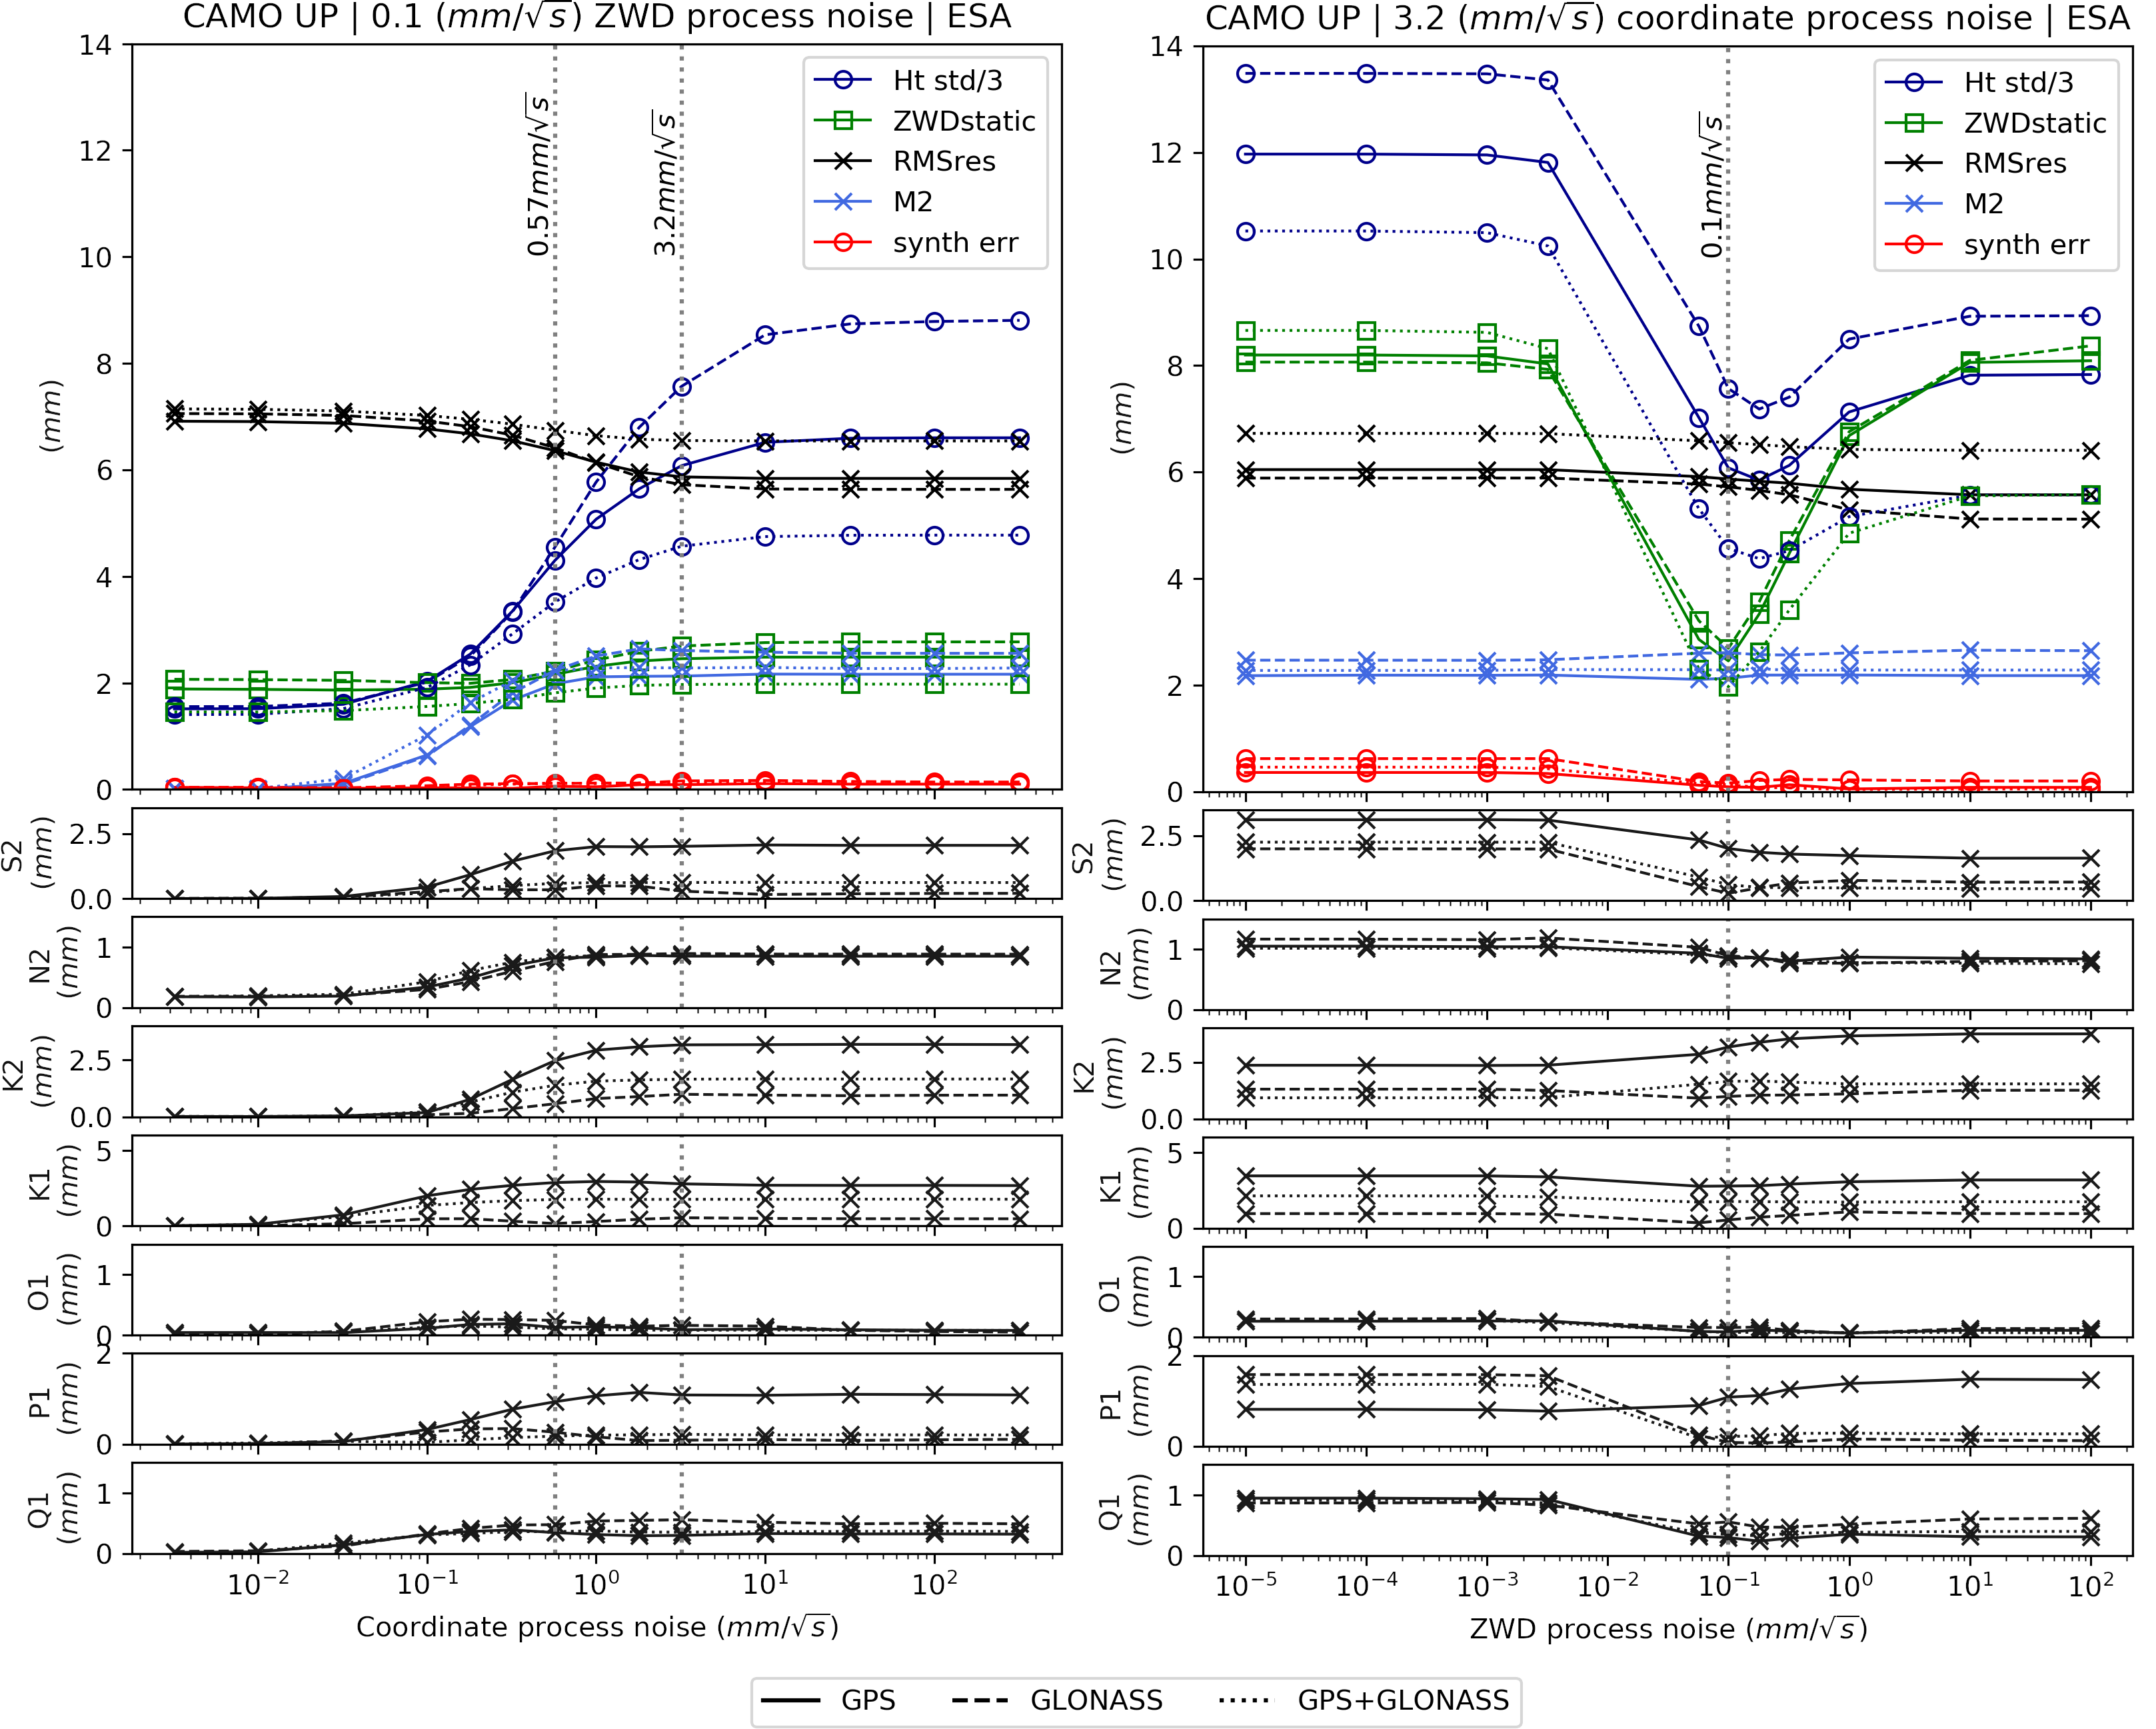
\includegraphics[width=17cm]{fig02.png}
\caption{The effect of varying coordinate process noise (left) and ZWD process noise (right) at test site CAMO for the up component (2010.0 – 2014.0), performed with ESA repro2 products. $\|Z_{res}\|$ is relative to FES2004\_GBe. The different constellations’ configurations: GPS, GLONASS and GPS+GLONASS are presented as solid, dashed and dotted lines respectively. The colours pertain to the different metrics as described in the text and legend (note the same scheme is used as per \cite{Penna2015}. }
\end{figure*}

For each of the major constituents, both diurnal and semi-diurnal, we found that 3.2 mm/sqrt(s) for coordinate process noise and 0.1 mm/sqrt(s) for tropospheric zenith delay process noise were optimal for our solutions, the same values as identified by \cite{Penna2015}. Figure 2 shows the results of the tests, with the left panel showing the result of varying coordinate process noise while ZWD process noise was held fixed (0.1 mm/sqrt(s), a default value) and the right panel the result of varying the ZWD process noise with coordinate process noise equal to the optimum value of 3.2 mm/sqrt(s). Same optimal process noise settings  for all constituents suggests that the different amplitudes and frequencies are less important than the data noise in the semidiurnal and diurnal frequency bands. 

\section{Results and Discussion}

%\subsection{Effect of using GLONASS}
Given the known accuracy of the ocean tide models in this region, and small effects of errors in solid Earth models, our assumption is that as $\|Z_{res}\|$ approaches zero as the estimates increase in accuracy, as in \cite{Bos2015}. Based on previous studies \citep[e.g.,][]{Yuan2013} we expected $\|Z_{res}\|$ median values (up) of $\sim$2 mm for $K_2$ and $K_1$, $\sim$1 mm for $M_2$, $S_2$, $P_1$ and $\sim$0.5 mm for $N_2$, $O_1$, $Q_1$. Figure 3 shows GPS, GLONASS and GPS+GLONASS $\|Z_{res}\|$ estimates for east, north and up coordinate components. The combined GPS+GLONASS solutions perform either at the same level as GPS AR ($M_2$, $O_1$, $Q_1$) or better ($N_2$, $P_1$) for the up component. $\|Z_{res}\|$ values are smaller and more consistent for the east ($M_2$, $N_2$, $O_1$) and north ($M_2$, $N_2$, $P_1$) components respectively. 
Also, the GPS+GLONASS solution does not have $\|Z_{res}\|$ biases in the east and north components as is noticeable for the GPS AR solution (particularly for $O_1$ in east, and $P_1$ in north, respectively). By $\|Z_{res}\|$ bias we mean a noticeable gap between zero and the lower whisker. 

%figure 3
\begin{figure*}[t]
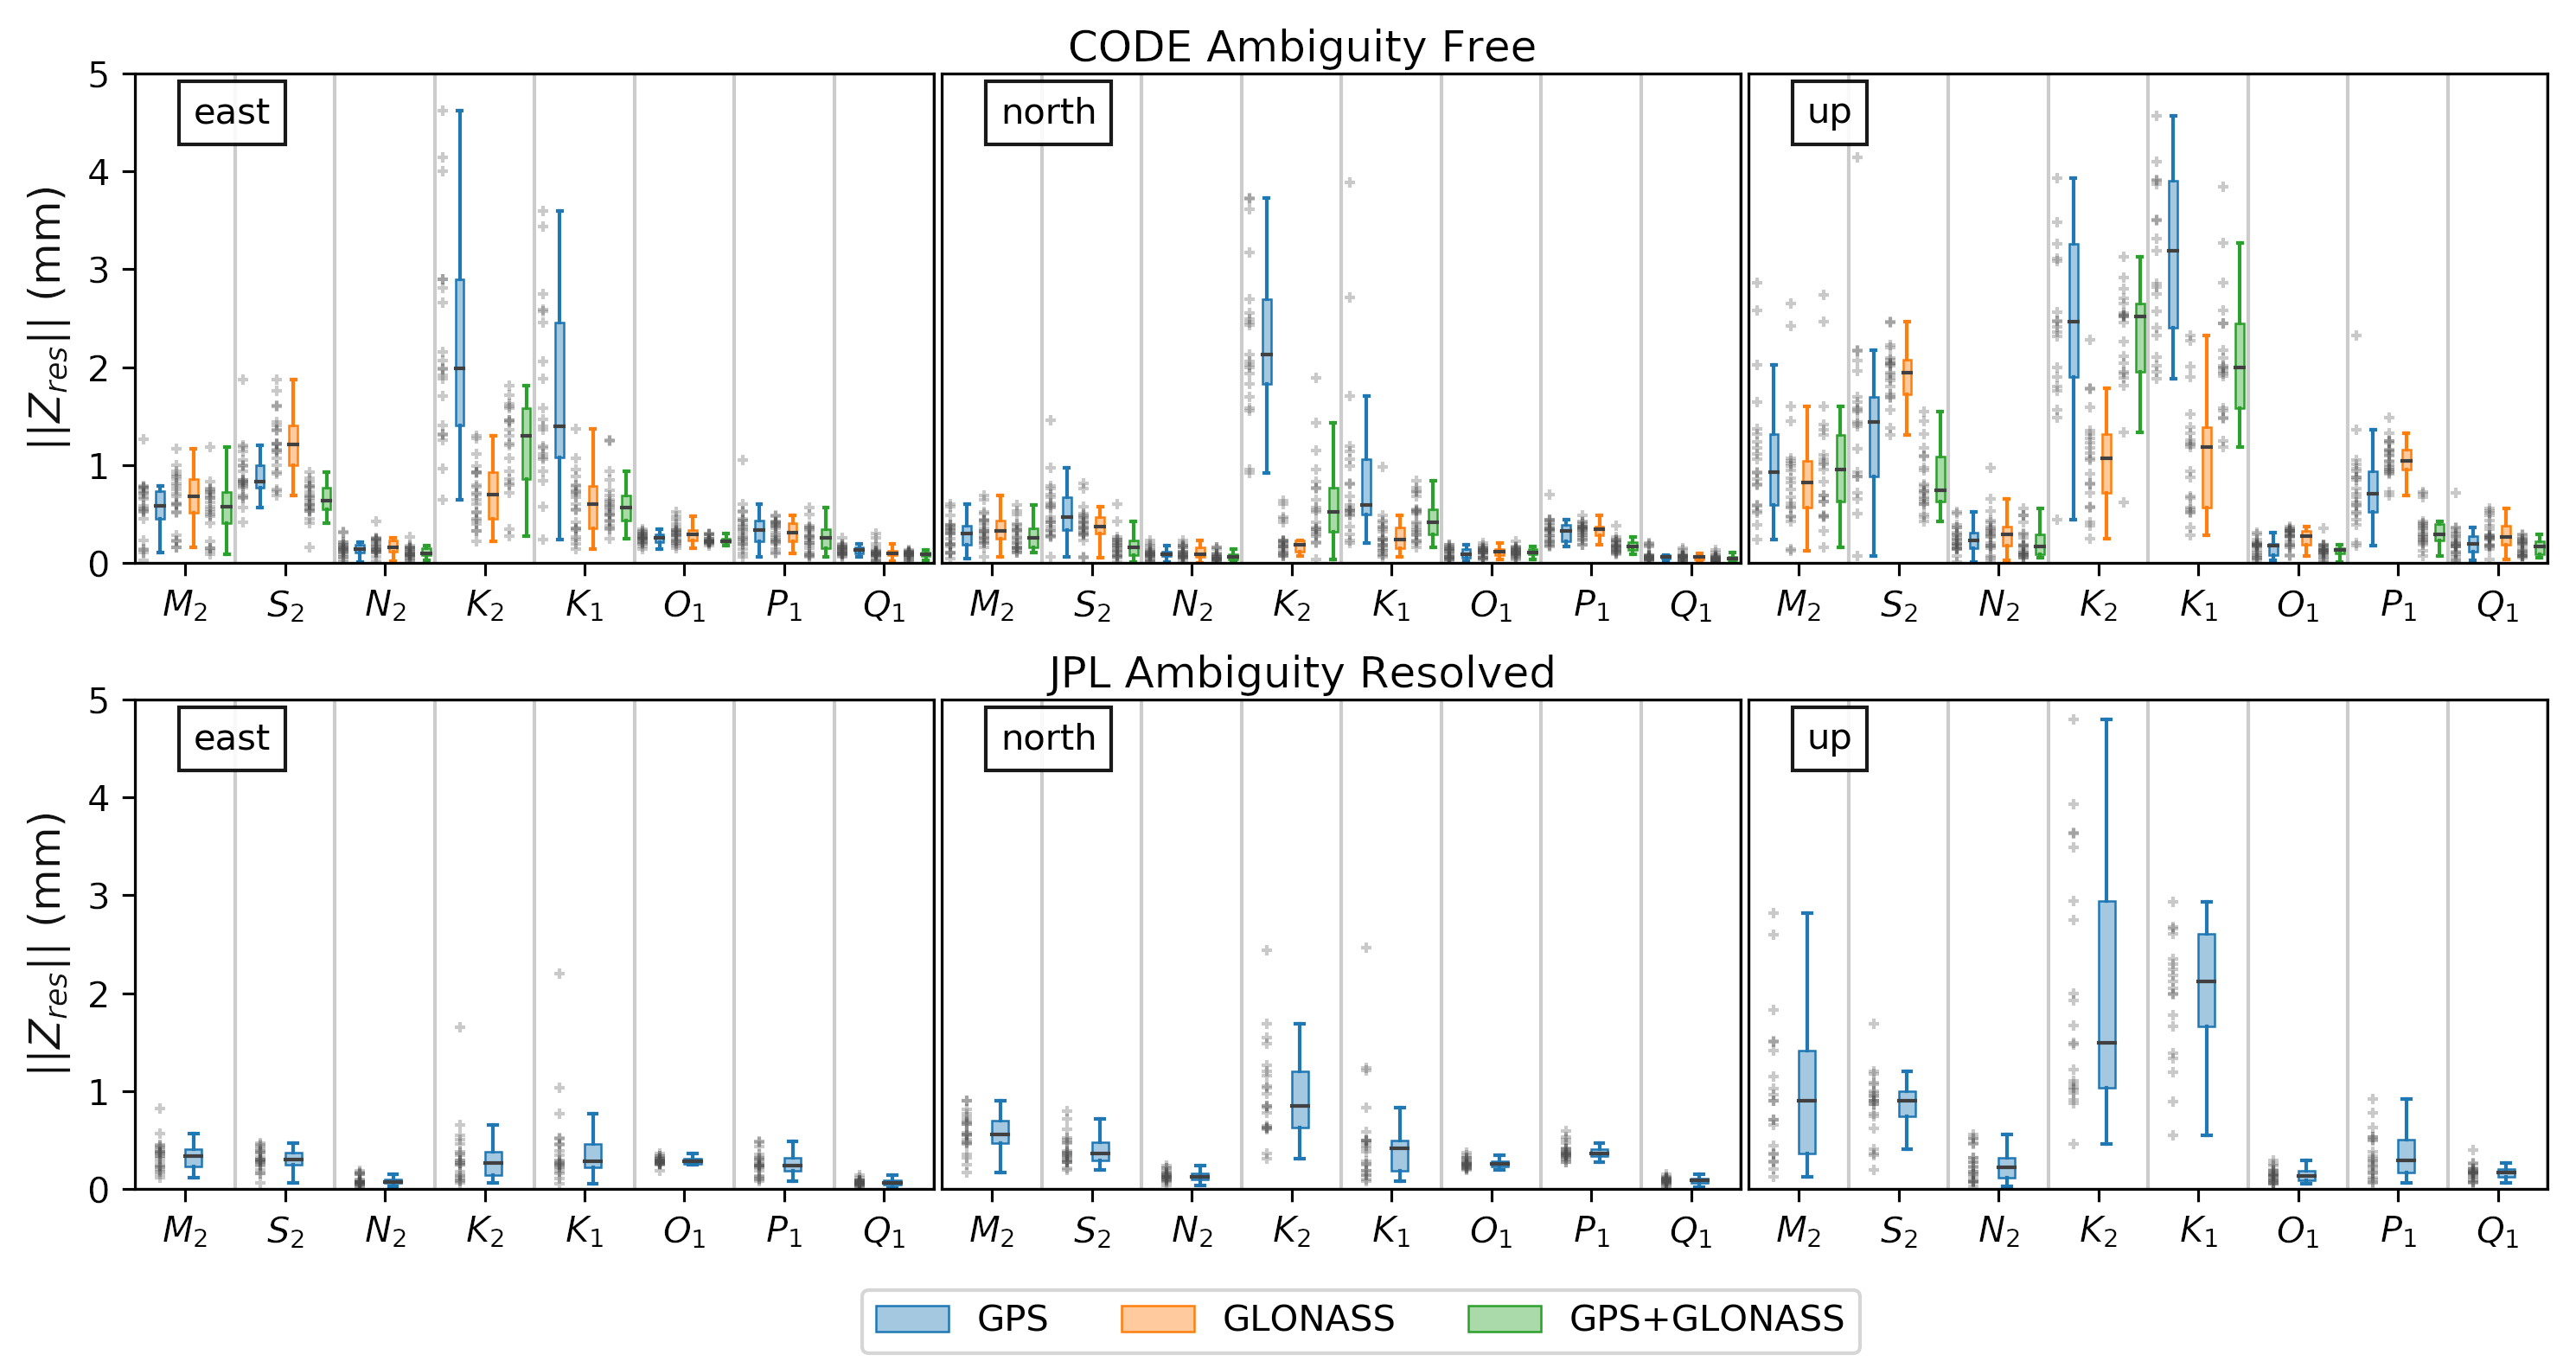
\includegraphics[width=17cm]{fig03.png}
\caption{$\|Z_{res}\|$ per tidal constituent for east, north and up components (left, middle and right, respectively) relative to FES2014b\_STW105d OTL values with CMC correction for JPL solutions. Grey crosses to the left of each boxplot represent sites’ $\|Z_{res}\|$ values and are offset horizontally for clarity while the horizontal line over each boxplot is a median of each constituent’s $\|Z_{res}\|$. Top: $\|Z_{res}\|$ for GPS, GLONASS and GPS+GLONASS PPP solutions (blue, orange and green, respectively) computed using CODE products. Bottom : $\|Z_{res}\|$ of the GPS AR solution computed with JPL native products.}
\end{figure*}

Considering the problematic GPS $K_2$ and $K_1$ constituents, the GPS AR can reasonably reliably, in comparison to other types of solutions, extract $\|Z_{res}\|$ in the east component (Figure 3, lower left panel) which is smaller than that of GLONASS and GPS+GLONASS using ESA or CODE products. However, smallest $\|Z_{res}\|$ extraction in the up and north components is possible only using GLONASS constellation solely.

Our results suggest that no single solution provides consistently better constituent estimates across all coordinate components. We suggest that optimum results are obtained using GPS+GLONASS for $M_2$, $N_2$, $O_1$, $P_1$ and $Q_1$, and GLONASS for $K_2$ and $K_1$, noting that GPS AR performs better for all constituents in the east component.

We now explore the sensitivity of our solutions to different products and analysis choices starting with elevation cutoff angle sensitivity, which particularly affects the amount of multipath influence on the coordinate time series. We follow with intercomparison of various products and assessing impact of integer ambiguity resolution (GPS only). Finally, we test the stability of the constituent estimates to time series length. 

\subsection{Satellite orbit and clock products sensitivity tests}
We assessed whether the solutions were sensitive to changes in satellite-elevation cutoff angle. Three additional cutoff angle scenarios were tested: 10°, 15° and 20° (in addition to the default 7° cutoff angle). Different elevation cutoffs will significantly alter the observation geometry as well as modulate the expression of signal multipath into solutions, decreasing its amount with higher cutoff value.

Figure 4 (top) shows the magnitude of vector difference, $\|\Delta Z_{res}\|$, between $Z_{res}$ values estimated from the 7° and 20° solutions and CODE products in both cases (upper subplot). $S_2$, $K_2$, $K_1$ and $P_1$ constituents in the up coordinate component show large mean magnitude of vector differences in both GPS (0.56, 2.29, 2.88, 0.54 mm, respectively) and GLONASS (0.82, 0.64, 1.01, 0.58 mm, respectively) with the rest of constituents showing differences of less than 0.5 mm. GPS+GLONASS shows smallest $\|\Delta Z_{res}\|$ between 7° and 20° estimates for $S_2$ and $P_1$ (0.31, 0.23 mm, respectively) and an additional decrease in $\|\Delta Z_{res}\|$ for $M_2$, $S_2$,$N_2$, $O_1$, $Q_1$ in the up component, which indicate higher closeness of compared OTL values – higher stability towards cutoff angle change.

%figure 4
\begin{figure*}[t]
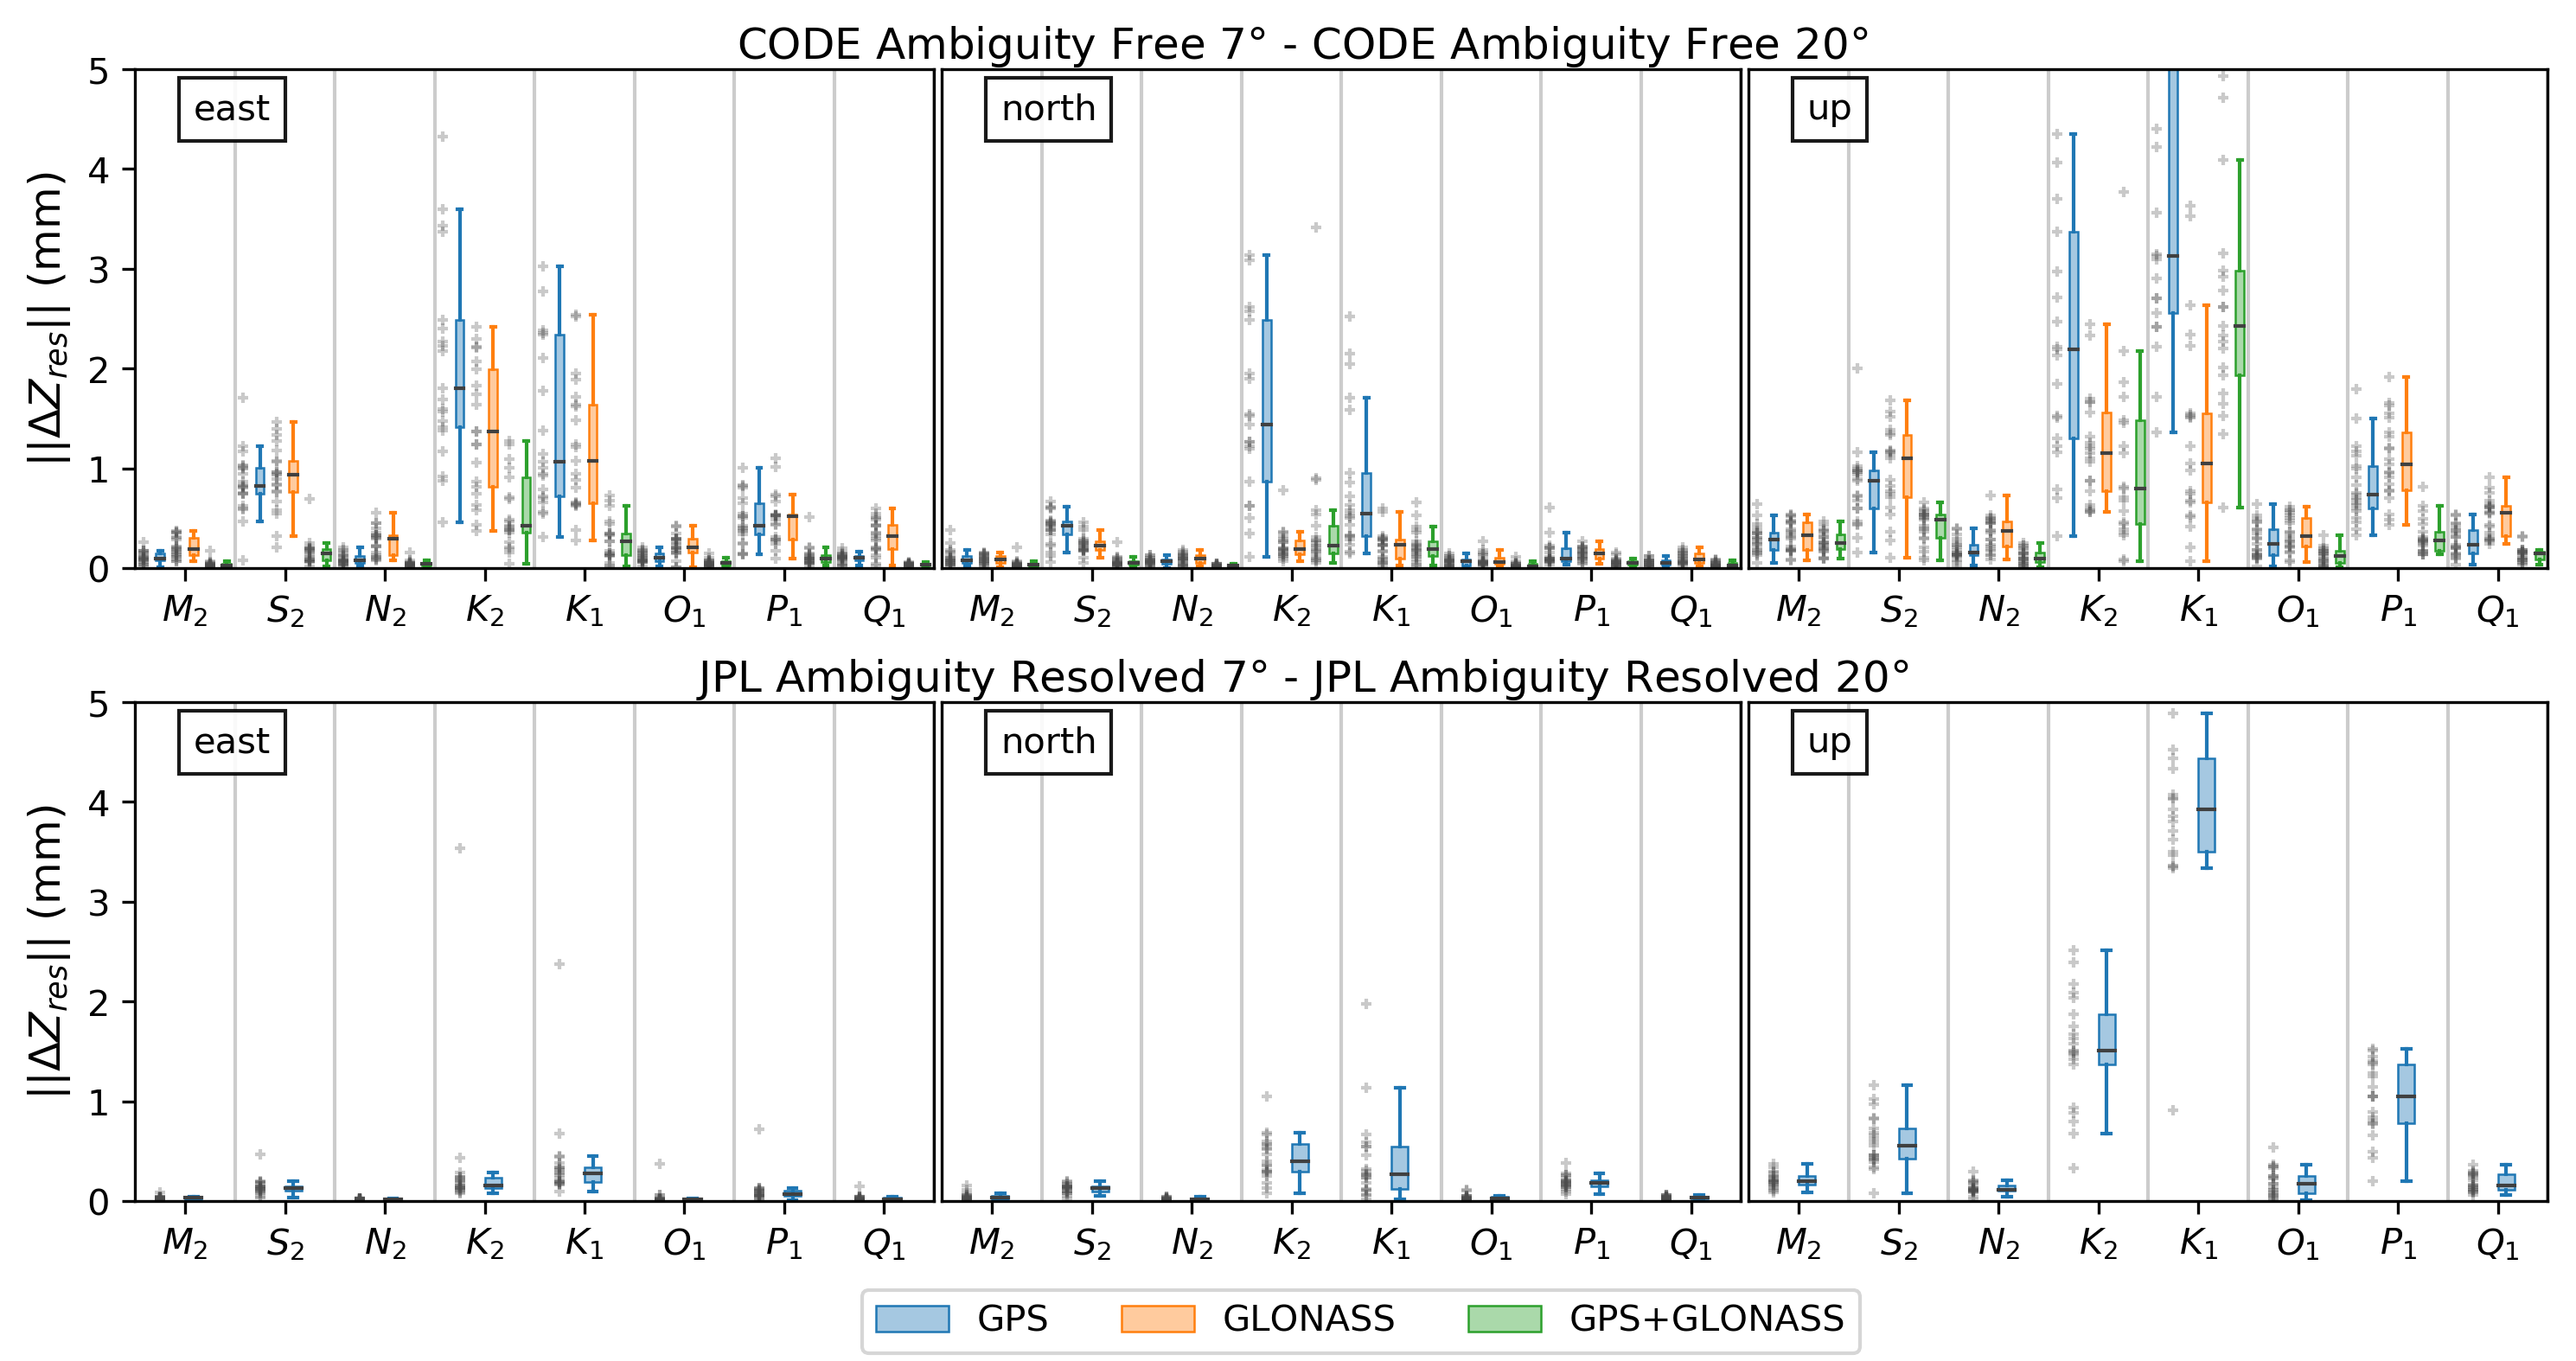
\includegraphics[width=17cm]{fig04.png}
\caption{Magnitude of vector difference between estimated $Z_{res}$ values computed with 7° and 20° elevation cutoff angles, $\|\Delta Z_{res}\|$, within the same set of orbits and clocks (top: CODE; bottom: JPL AR ) for east, north and up coordinate components (left, middle and right, respectively). Grey crosses are as per figure 3. The smaller residuals using CODE products with GPS+GLONASS (top) is a result of improved OTL stability as a function of cutoff angle using combined constellations (except $K_1$ up and $K_2$ up). JPL’s GPS AR also shows great stability with exception of $K_2$ up and $K_1$ up. $\|\Delta Z_{res}\|$ for GPS, GLONASS and GPS+GLONASS PPP solutions in blue, orange and green, respectively.}
\end{figure*}

The same comparison done for GPS AR (7° and 20° cutoff, JPL native products) shows largely improved stability in comparison to all GPS only ambiguity free solutions (Figure 4, bottom). However, $K_2$ up and $K_1$ up show substantial differences between solutions: $K_2$ shows as much smaller variance of $\|Z_{res}\|$ distribution in the 20° solution, possibly due to removal of multipath, and $K_1$ shows an increased dispersion and median of $\|Z_{res}\|$ at increased cutoff angle.

Following \cite{Yuan2013}, we assessed the possible influence of inconsistencies in precomputed orbits/clocks on estimated OTL displacements. This was done by computing $\|\Delta Z_{res}\|$ between pairs of solutions with common constellation configurations: GPS (no AR here) solutions computed using ESA, CODE and JPL products; GLONASS/GPS+GLONASS solutions using ESA and CODE products.

Figure 5 (top) shows the distribution of $\|\Delta Z_{res}\|$ between solutions computed with ESA and CODE products for all three constellation modes: GPS, GLONASS and GPS+GLONASS. The main differences are related to the $S_2$, $K_2$, $K_1$ and $P_1$ constituents. The maximum $\|\Delta Z_{res}\|$ between the observed OTL for the rest of the constituents is less than $\sim$0.3 mm.

Compared with GPS JPL, both CODE and ESA solutions (Figure 5, middle and bottom, respectively) show $\|\Delta Z_{res}\|$ up to 0.5 mm in the horizontal components with respect to JPL solutions, which is also true for ESA in the up component with exception for $K_2$ and $K_1$. CODE shows similar behaviour to ESA, however, significant divergence from JPL (Figure 5, middle) is also observed for $S_2$ with even higher $\|\Delta Z_{res}\|$ for $K_2$ and $K_1$ in the up and the east.

%figure 5
\begin{figure*}[t]
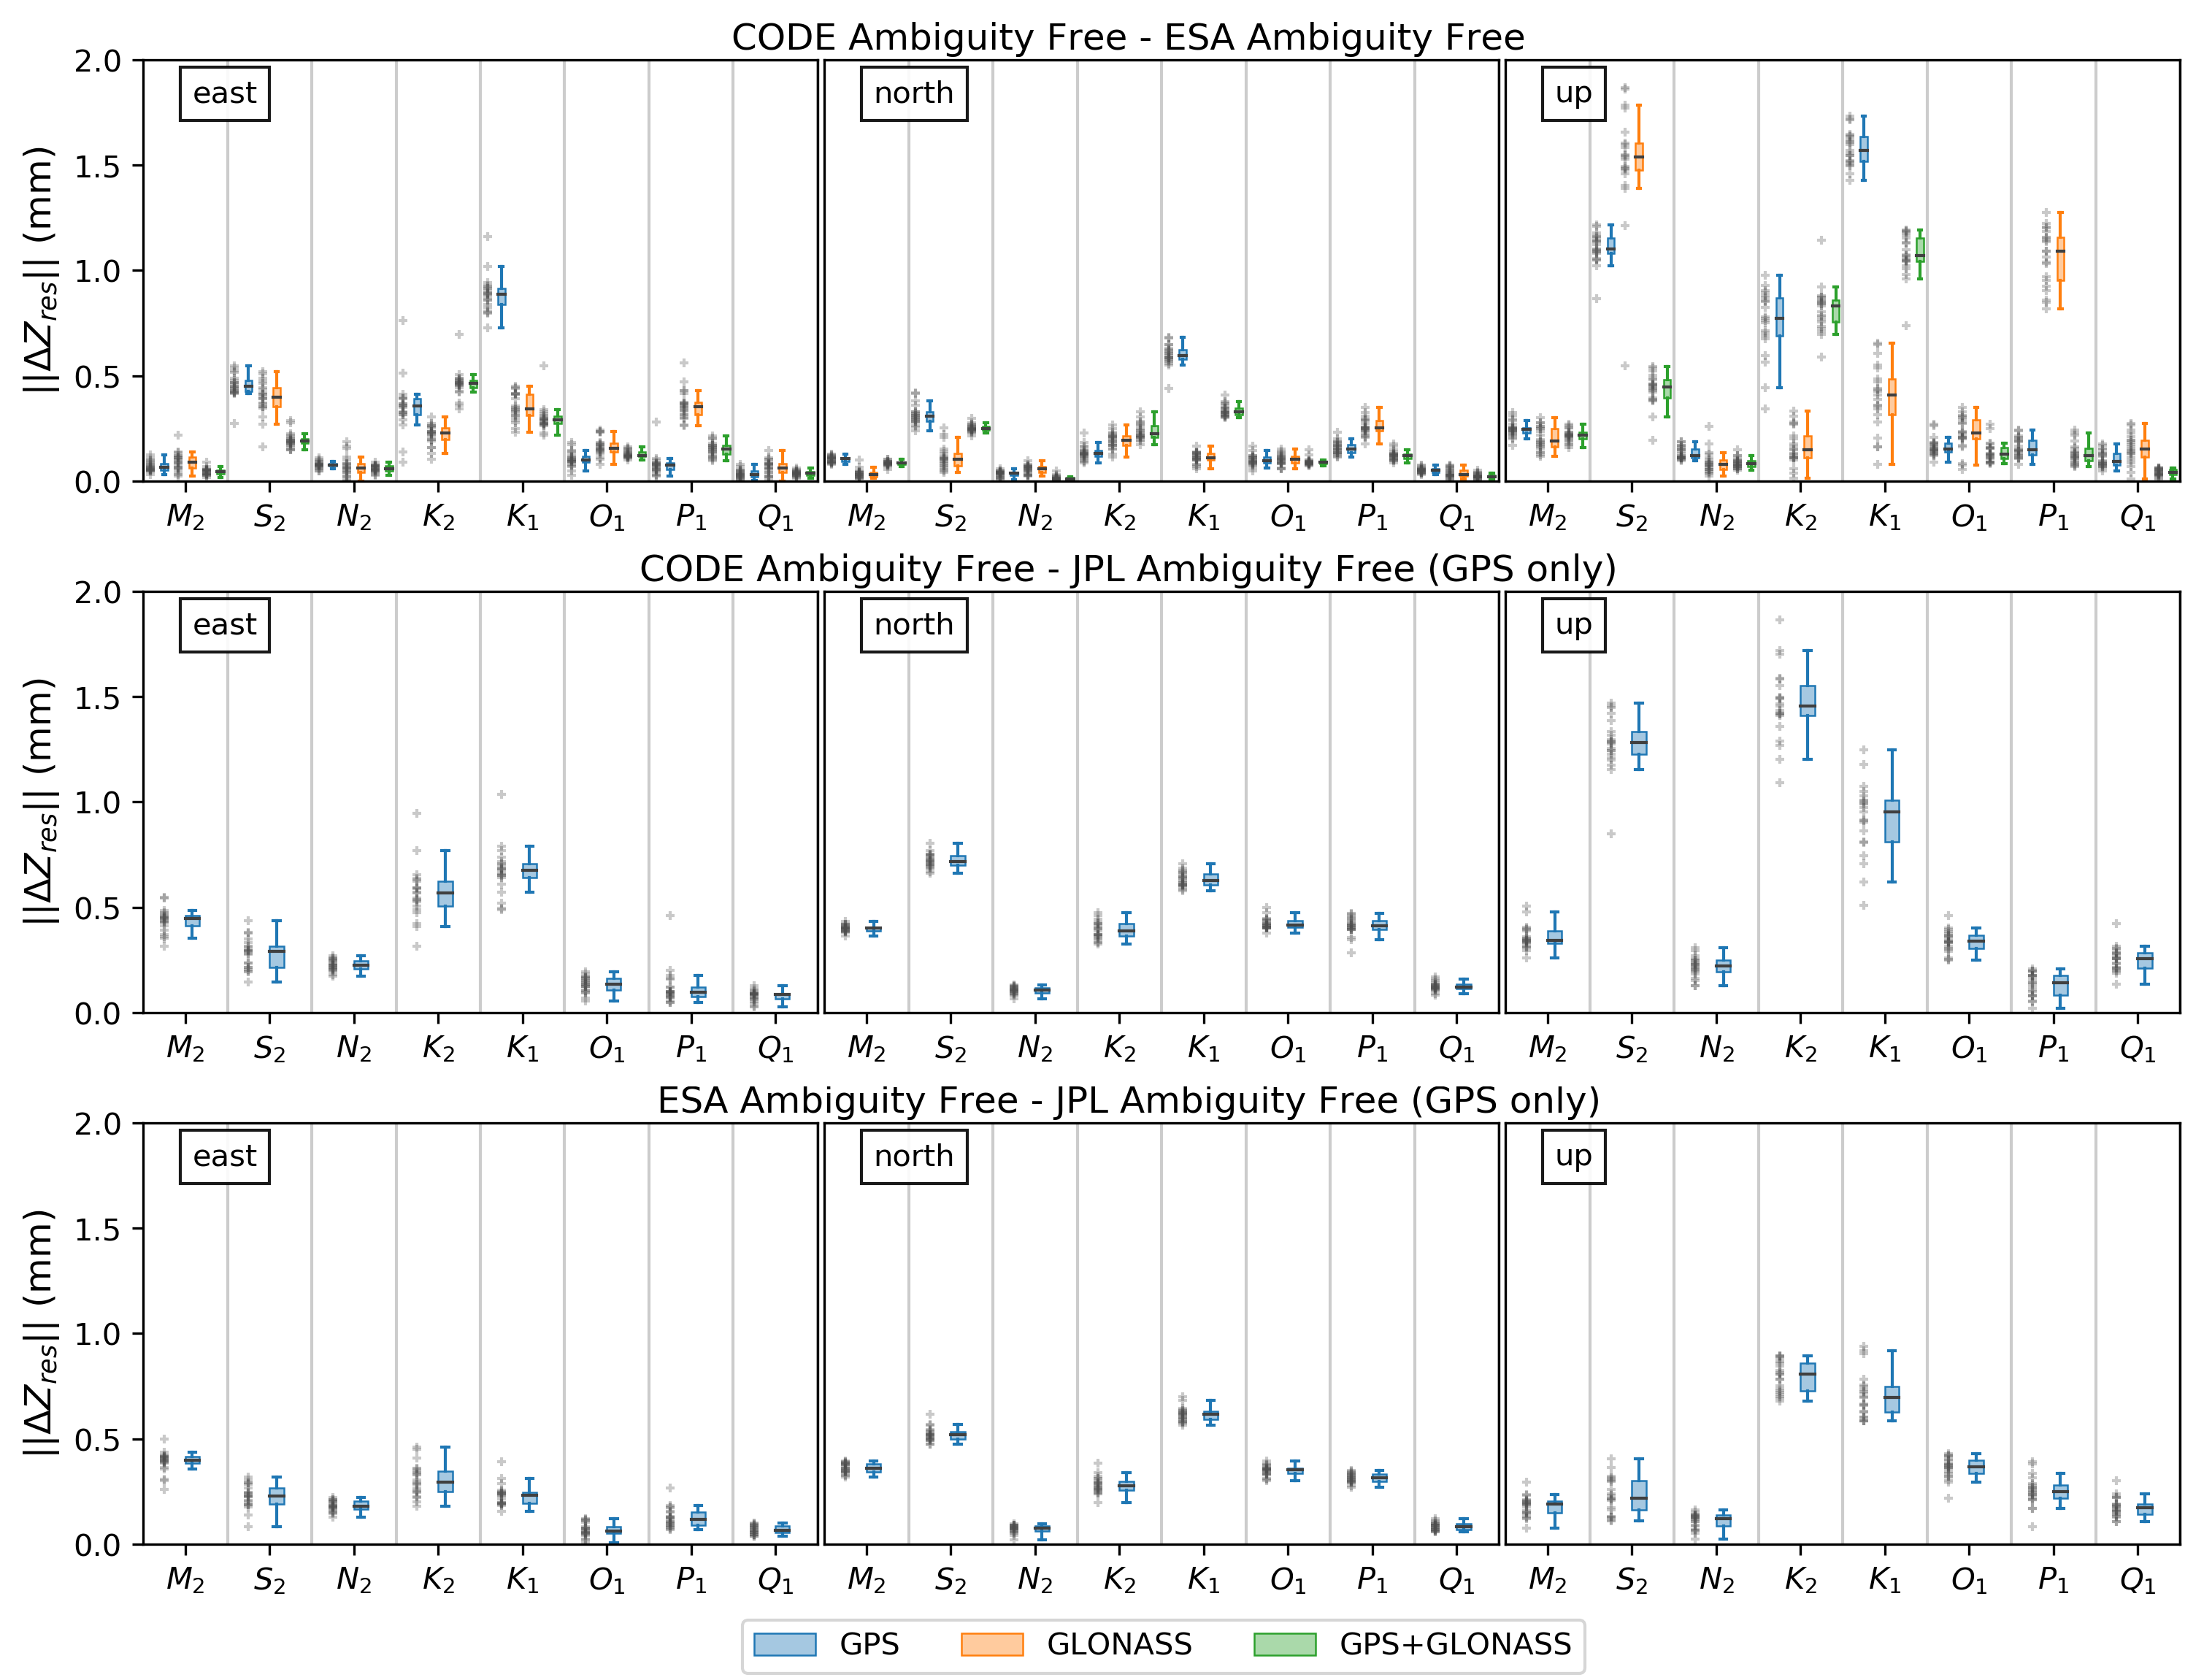
\includegraphics[width=17cm]{fig05.png}
\caption{OTL vector differences between CODE, ESA and JPL solutions (ambiguity free). Top: GPS, GLONASS and combined GPS+GLONASS differences between CODE and ESA solutions; Middle: GPS difference between CODE and JPL solutions (ambiguity free); Bottom: GPS difference between ESA and JPL solutions (ambiguity free). Note the vertical scale of 2 mm. Grey crosses are as per Figure 3. }
\end{figure*}

\subsection{$S_2$ constituent}
Focusing on $S_2$, the GPS up residual shows $\sim$1 mm residual bias between solutions using CODE and ESA products (compare blue records between left and right panels, Figure 6). The GPS $\|Z_{res}\|$ bias is maintained for solutions with a range of elevation cutoff angles (7°, 10°, 15° and 20°). GLONASS solutions (orange), however, show no $\|Z_{res}\|$ bias for ESA and $\sim$1.5 mm bias for CODE, both with 7 ° elevation angle. GLONASS bias values in both cases increase with elevation cutoff angle up to 15°. This GLONASS dependency with elevation cutoff is present to a lesser degree in both east and north components and is the same with ESA and CODE products (Fig. S5).

%figure 6
\begin{figure}[t]
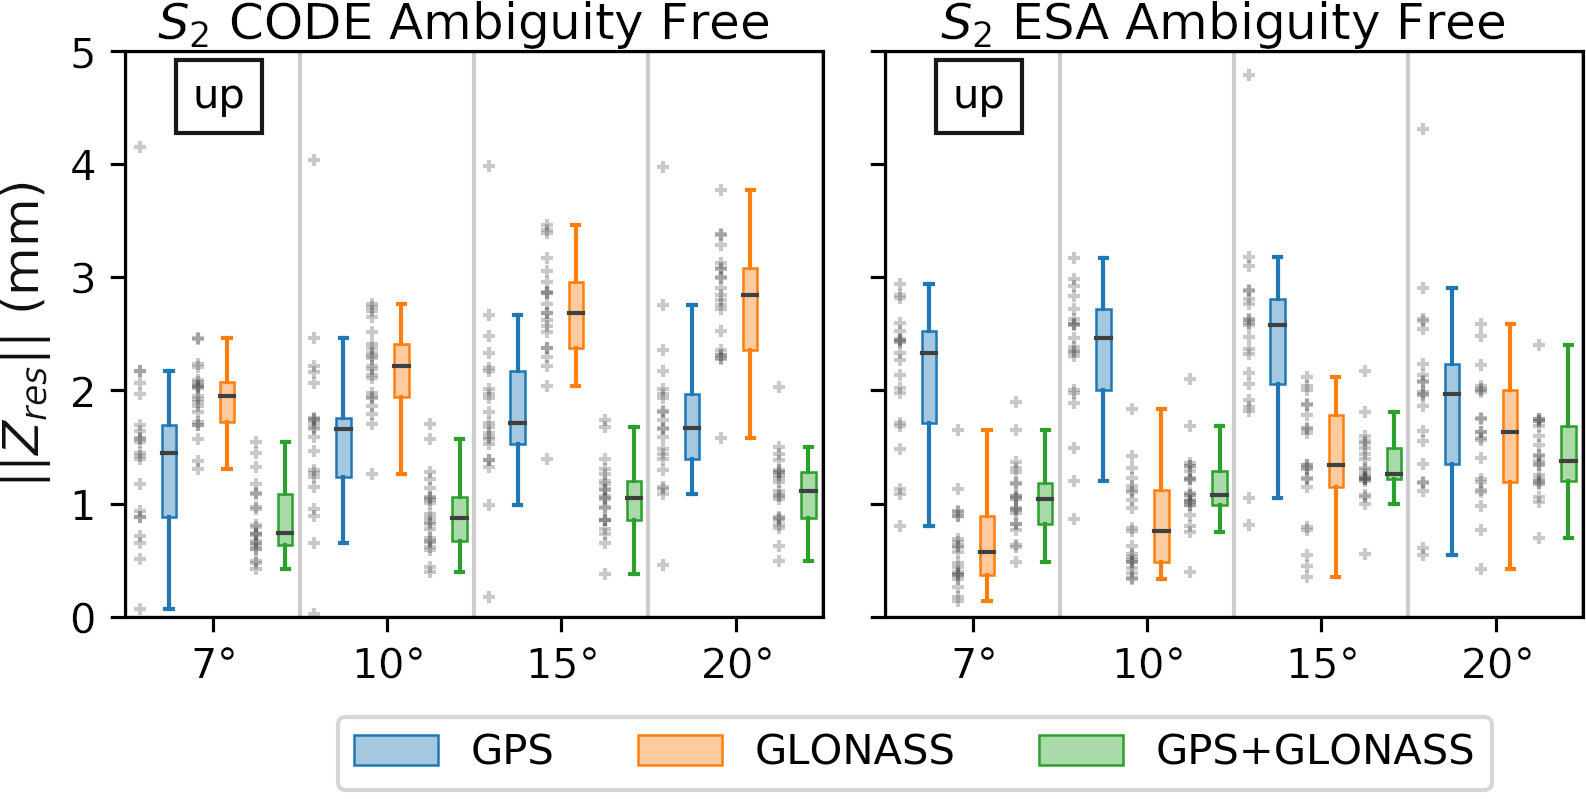
\includegraphics[width=8.3cm]{fig06.png}
\caption{GPS, GLONASS and GPS+GLONASS $\|Z_{res}\|$ for the $S_2$ constituent in the up component as a function of elevation cutoff angle, computed with ESA (left) and CODE products (right). Note the inverse behaviour of GPS and GLONASS biases and the linear dependence of the GLONASS biases. Grey crosses are as per Fig. 3.}
\end{figure}

GPS $\|Z_{res}\|$ estimates show similar behaviour in terms of $\|Z_{res}\|$ bias between ESA and CODE solutions in the up component (blue, Figure 6) but ESA solutions' median $\|Z_{res}\|$ values are $\sim$1 mm larger for all elevation cutoff angle solutions.
Both ESA and CODE GPS+GLONASS $S_2$ results (green, Figure 6) show a blend of the two patterns observed with GPS and GLONASS solutions. GPS+GLONASS $S_2$ shows less sensitivity to the cutoff angle change than GLONASS or GPS solutions with both products. The effect was also studied with JPL products and AR: GPS and GPS AR; see Sect. 5.7.

The substantial difference in $S_2$ between ESA and CODE (Figure 6) suggests important differences in raw GNSS data analysis approaches within respective Analysis Centres. One relevant difference between products is in treatment of $S_1$ and $S_2$ atmospheric tides which were corrected for at the observation level in CODE products but not in ESA. However, the inverse behaviour of GPS and GLONASS between ESA and CODE solutions (orange, Figure 6) cannot be explained with a single correction applied to both constellations. We expect that the differences in each solution are a function of satellite orbit modelling, although the issue is not clear and needs further investigation.


\subsection{$K_2$ and $K_1$ constituents}
As seen from Fig. 3, $\| Z_{res}\|$ can be minimized if using GLONASS for the extraction of $K_1$ and $K_2$ constituents and GPS+GLONASS for the remainder of the constituents. In this case, $\| Z_{res}\|$ will stay below 0.25 mm for north components and below 0.5 mm for the east and the up components.

GLONASS $K_2$ and $K_1$ estimates in the north have lowest variance in $\|Z_{res}\|$ and most stable with different elevation cutoff angles and products. For the east component, CODE products with GLONASS struggle to compete with GPS+GLONASS in terms of $\|Z_{res}\|$ distribution variance ($K_1$) and elevation cutoff stability ($K_2$ and $K_1$). The ESA products GLONASS, however, performs better for $K_1$ east than the respective GPS+GLONASS in terms of $\|Z_{res}\|$ distribution consistency and median (Fig. S2). Elevation cutoff stability of ESA $K_2$ and $K_1$ in the east component is exactly as with CODE – best with GPS+GLONASS.

The up component of $K_2$ and $K_1$ is the most problematic, showing high $\|Z_{res}\|$ values with all constellation modes. GLONASS OTL values from both ESA and CODE solutions have the smallest $\|Z_{res}\|$ distribution variances and median values outperforming JPL GPS AR. Note that GPS+GLONASS $K_2$ up has a marginally smaller median $\|\Delta Z_{res}\|$ in the elevation cutoff test, possibly due to the larger number of total satellites, however, both $K_2$ and $K_1$ $\|Z_{res}\|$ posses \sim1.5 mm bias.

While we cannot certainly select a single constellation configuration optimal for all components of $K_2$ and $K_1$, we can conclude that based on our analysis, GLONASS returns smaller $\|Z_{res}\|$ in the $K_2$ and $K_1$ north and up components while east component might show better results with GPS+GLONASS ($K_1$, CODE) but, due to great agreement between products, solutions using GLONASS constellation are still preferred. The only exception to the east component conclusions is GPS AR (see Sect. 5.7).

\subsection{$P_1$ constituent}
The high $\|\Delta Z_{res}\|$ in GLONASS $P_1$ constituent between CODE and ESA solutions over all coordinate components (orange, Figure 5 top) is unexpected as ESA and CODE $\|Z_{res}\|$ boxplots show similar distributions of values (see Figure S2 in the supplementary material for the equivalent ESA boxplots). This suggests a symmetrical deviation from the modelled values that produces a high $\|\Delta Z_{res}\|$. In all cases, however, GPS+GLONASS is preferred for $P_1$ estimation.

\subsection{Effect of different orbit and clock products on noise and uncertainty}

%figure 7
\begin{figure}[t]
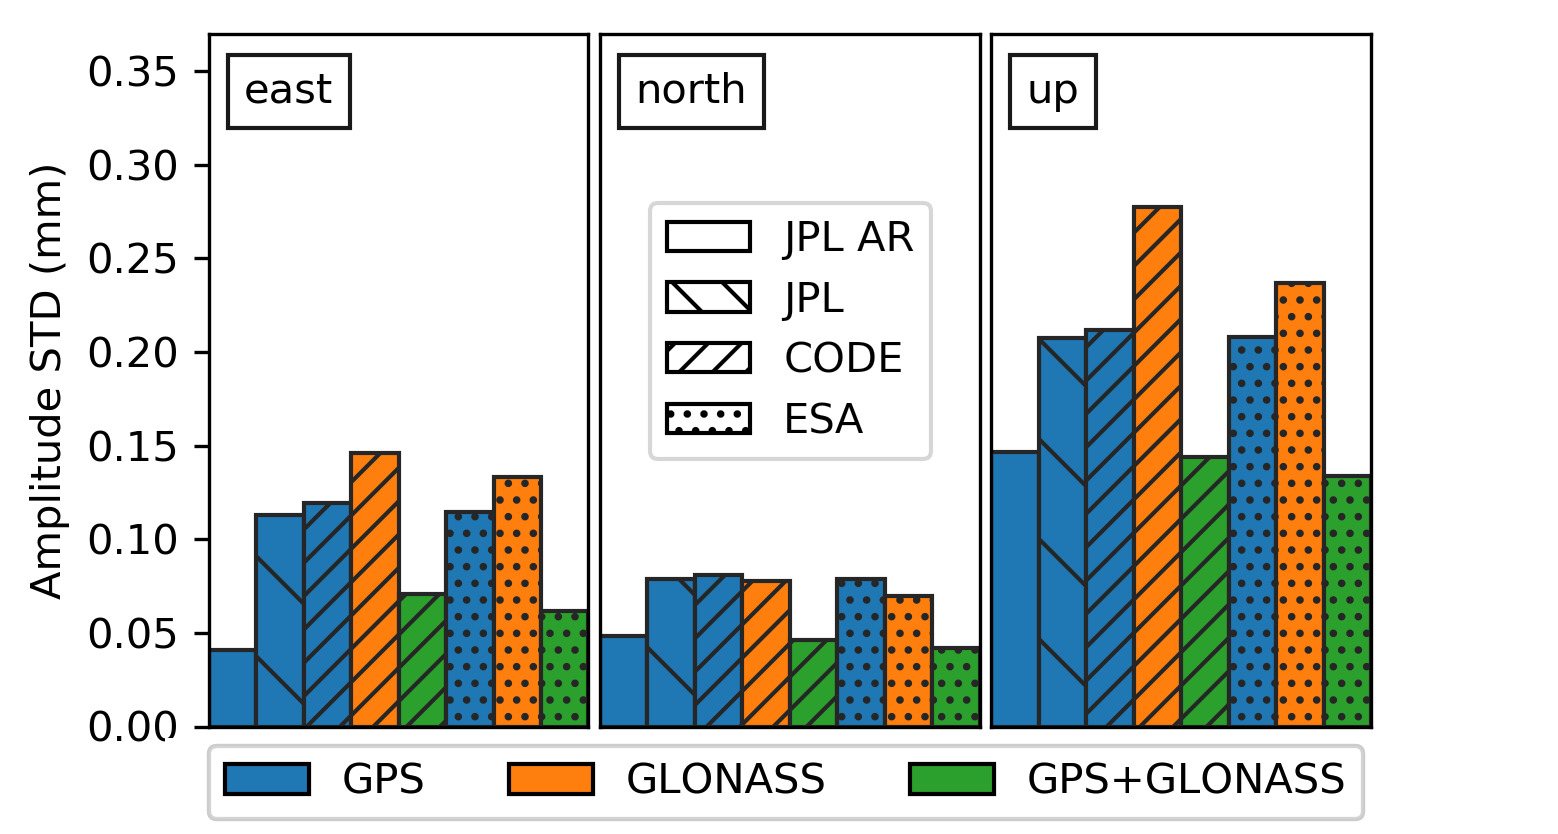
\includegraphics[width=8.3cm]{fig07.png}
\caption{Average uncertainties (1-sigma) for OTL amplitudes computed across eight OTL constituents per products (stipple) and processing modes/constellation (colour): GLONASS (orange) and GPS (blue) modes show higher uncertainties STDs, while GPS-only AR and combined GPS+GLONASS (green) show minimum uncertainties with exception for east.}
\end{figure}

Changing orbit and clock products also changes the time series noise characteristics and hence influences the uncertainties of the estimated constituents (estimated separately by Eterna for amplitude, Figure 7 and phase, Figure 8). Amplitude uncertainties are expressed here as an average across all constituents as they do not differ much between analysed constituents. ETERNA assumes a white noise model in its analysis. We conclude that GLONASS solutions produce the highest amplitude uncertainties for east (0.15 mm CODE, 0.14 mm ESA) and up components (0.22 mm CODE, 0.27mm ESA) while showing the same uncertainty as GPS for the north (0.07 mm, both CODE and ESA). GLONASS amplitude uncertainties from solutions using CODE products tend to be marginally higher than those of ESA products. The amplitude uncertainties for combined GPS+GLONASS solutions are equal to those of JPL with ambiguities fixed (GPS AR), although the JPL GPS AR solution has slightly smaller uncertainty in the east component (smaller by $\sim$0.02 mm).


Considering the uncertainties of phase values, these are unsurprisingly dependent on the constituent’s amplitude. JPL native products show a significant advantage in this case when compared to ESA and CODE due to differences in frames: CM (JPL) and CE (ESA and CODE). This results in up to an order of magnitude increase in phase uncertainties for “weaker” diurnal constituents in the region: $N_2$, $O_1$, $P_1$, $Q_1$ (Figure 8).

In general, this frame effect is directly related to centre of mass correction (CMC) specific to the constituent's CMC vector in comparison to the total theoretical OTL vector. If applying a CMC correction to the constituent increases its amplitude, phase STD values will decrease in a CM frame solution. This is critically important for the constituents with amplitudes below 0.5 mm, as phase uncertainty increases significantly below this threshold. The most significant exception in our dataset is $P_1$ in the up component which has a much larger amplitude in CE frame (Figure 8, right in top and bottom). 

%figure 8
\begin{figure*}[t]
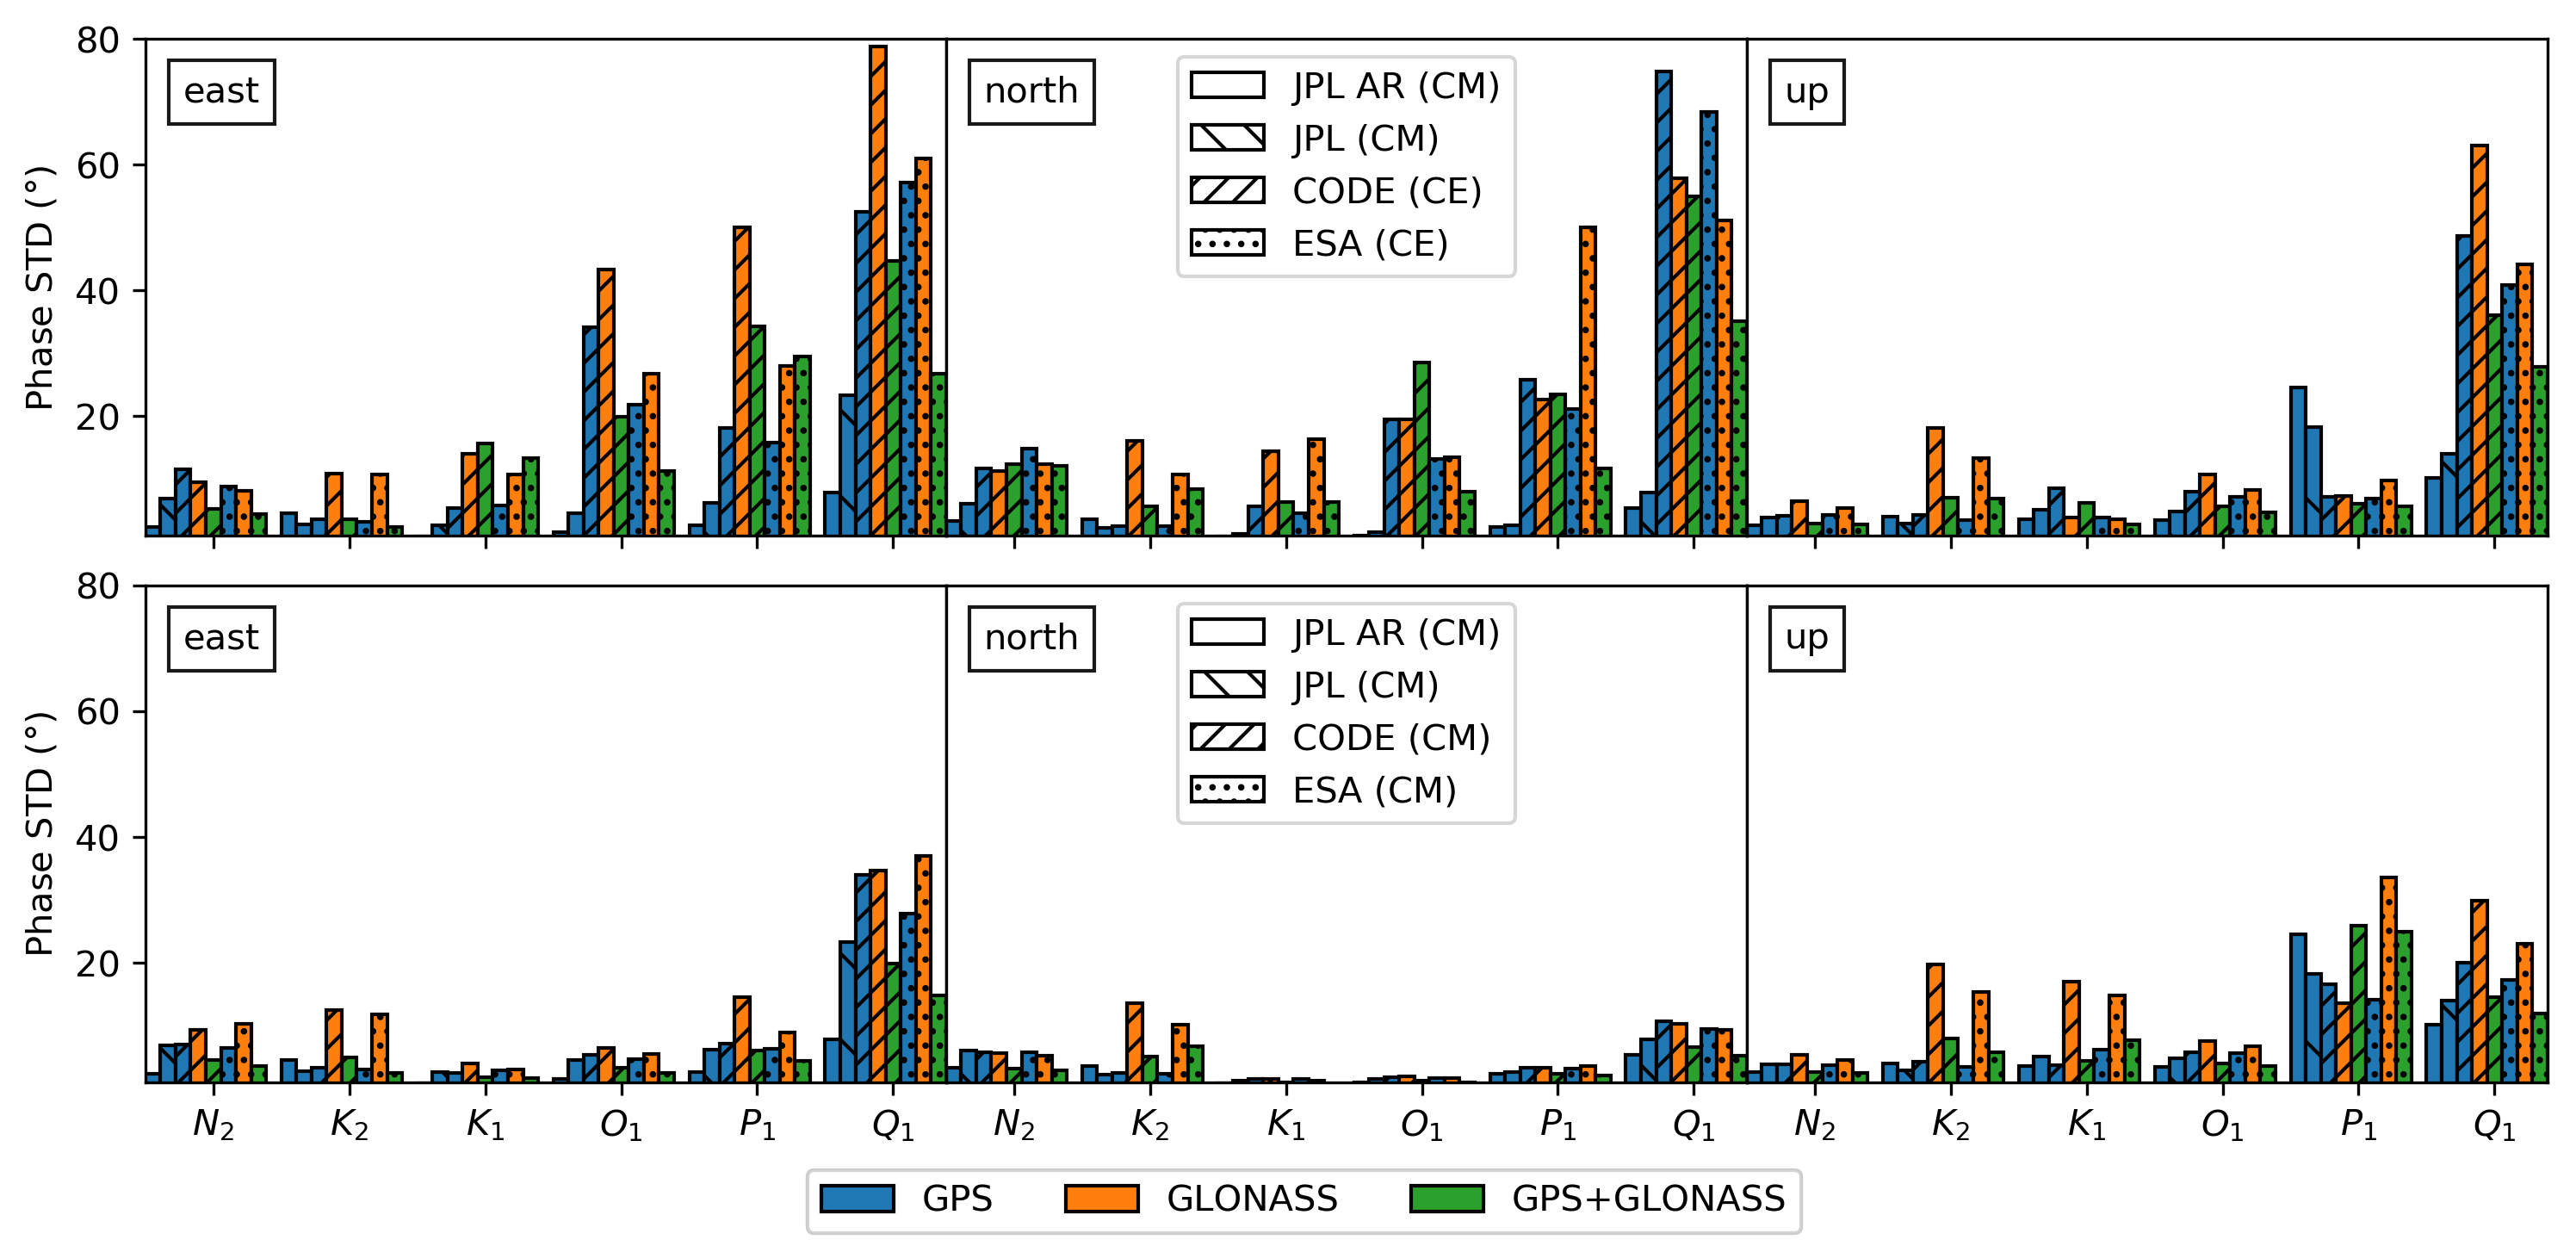
\includegraphics[width=17cm]{fig08.png}
\caption{Average phase STD (uncertainty) per constituent for different products as returned by Eterna. ESA and CODE products were in CE frame by default (top) and converted to CM (bottom) while JPL are in CM in both. $M_2$ and $S_2$ phase STDs are not shown here as values are too small to be seen with the scale specified.}
\end{figure*}

Converting CE products to CM (Figure 8, bottom) was done to demonstrate that the changes in phase uncertainty are indeed introduced by the smaller amplitudes in the CE frame. While this holds true, it is obvious that the $P_1$ up phase uncertainty increases, as was expected based on comparison with the JPL solutions. GLONASS $K_1$ up phase uncertainties show almost an order of magnitude increase in the CM frame while having unexpectedly small values in CE. This is a direct cause of GLONASS solution having larger $K_1$ up amplitudes in CE and smaller in CM with both CODE and ESA.

\subsection{Impact of Ambiguity Resolution on GPS}
The multi-GNSS products used here do not allow integer AR with PPP and this is an active area of research and development within the IGS. However, assessing the impact of AR on GPS-only solutions provides some insight towards the future benefit of AR on GLONASS and GPS+GLONASS solutions once such products become available. We compared OTL residuals from GPS and GPS AR using JPL native products that contain wide lane and phase bias tables (WLPB files) required for integer AR with PPP.

Figure 9 shows the effect on estimated constituents from enabling AR in a standard solution with 7° cutoff. Here we observe decreased $\|Z_{res}\|$ over all coordinate components compared with the estimates from a non-AR solution. This is most visible in the $K_2$ and $K_1$ constituents and in the elimination of the $S_2$ $\|Z_{res}\|$ bias and with smaller improvements in $M_2$ and $P_1$.

%figure 9
\begin{figure*}[t]
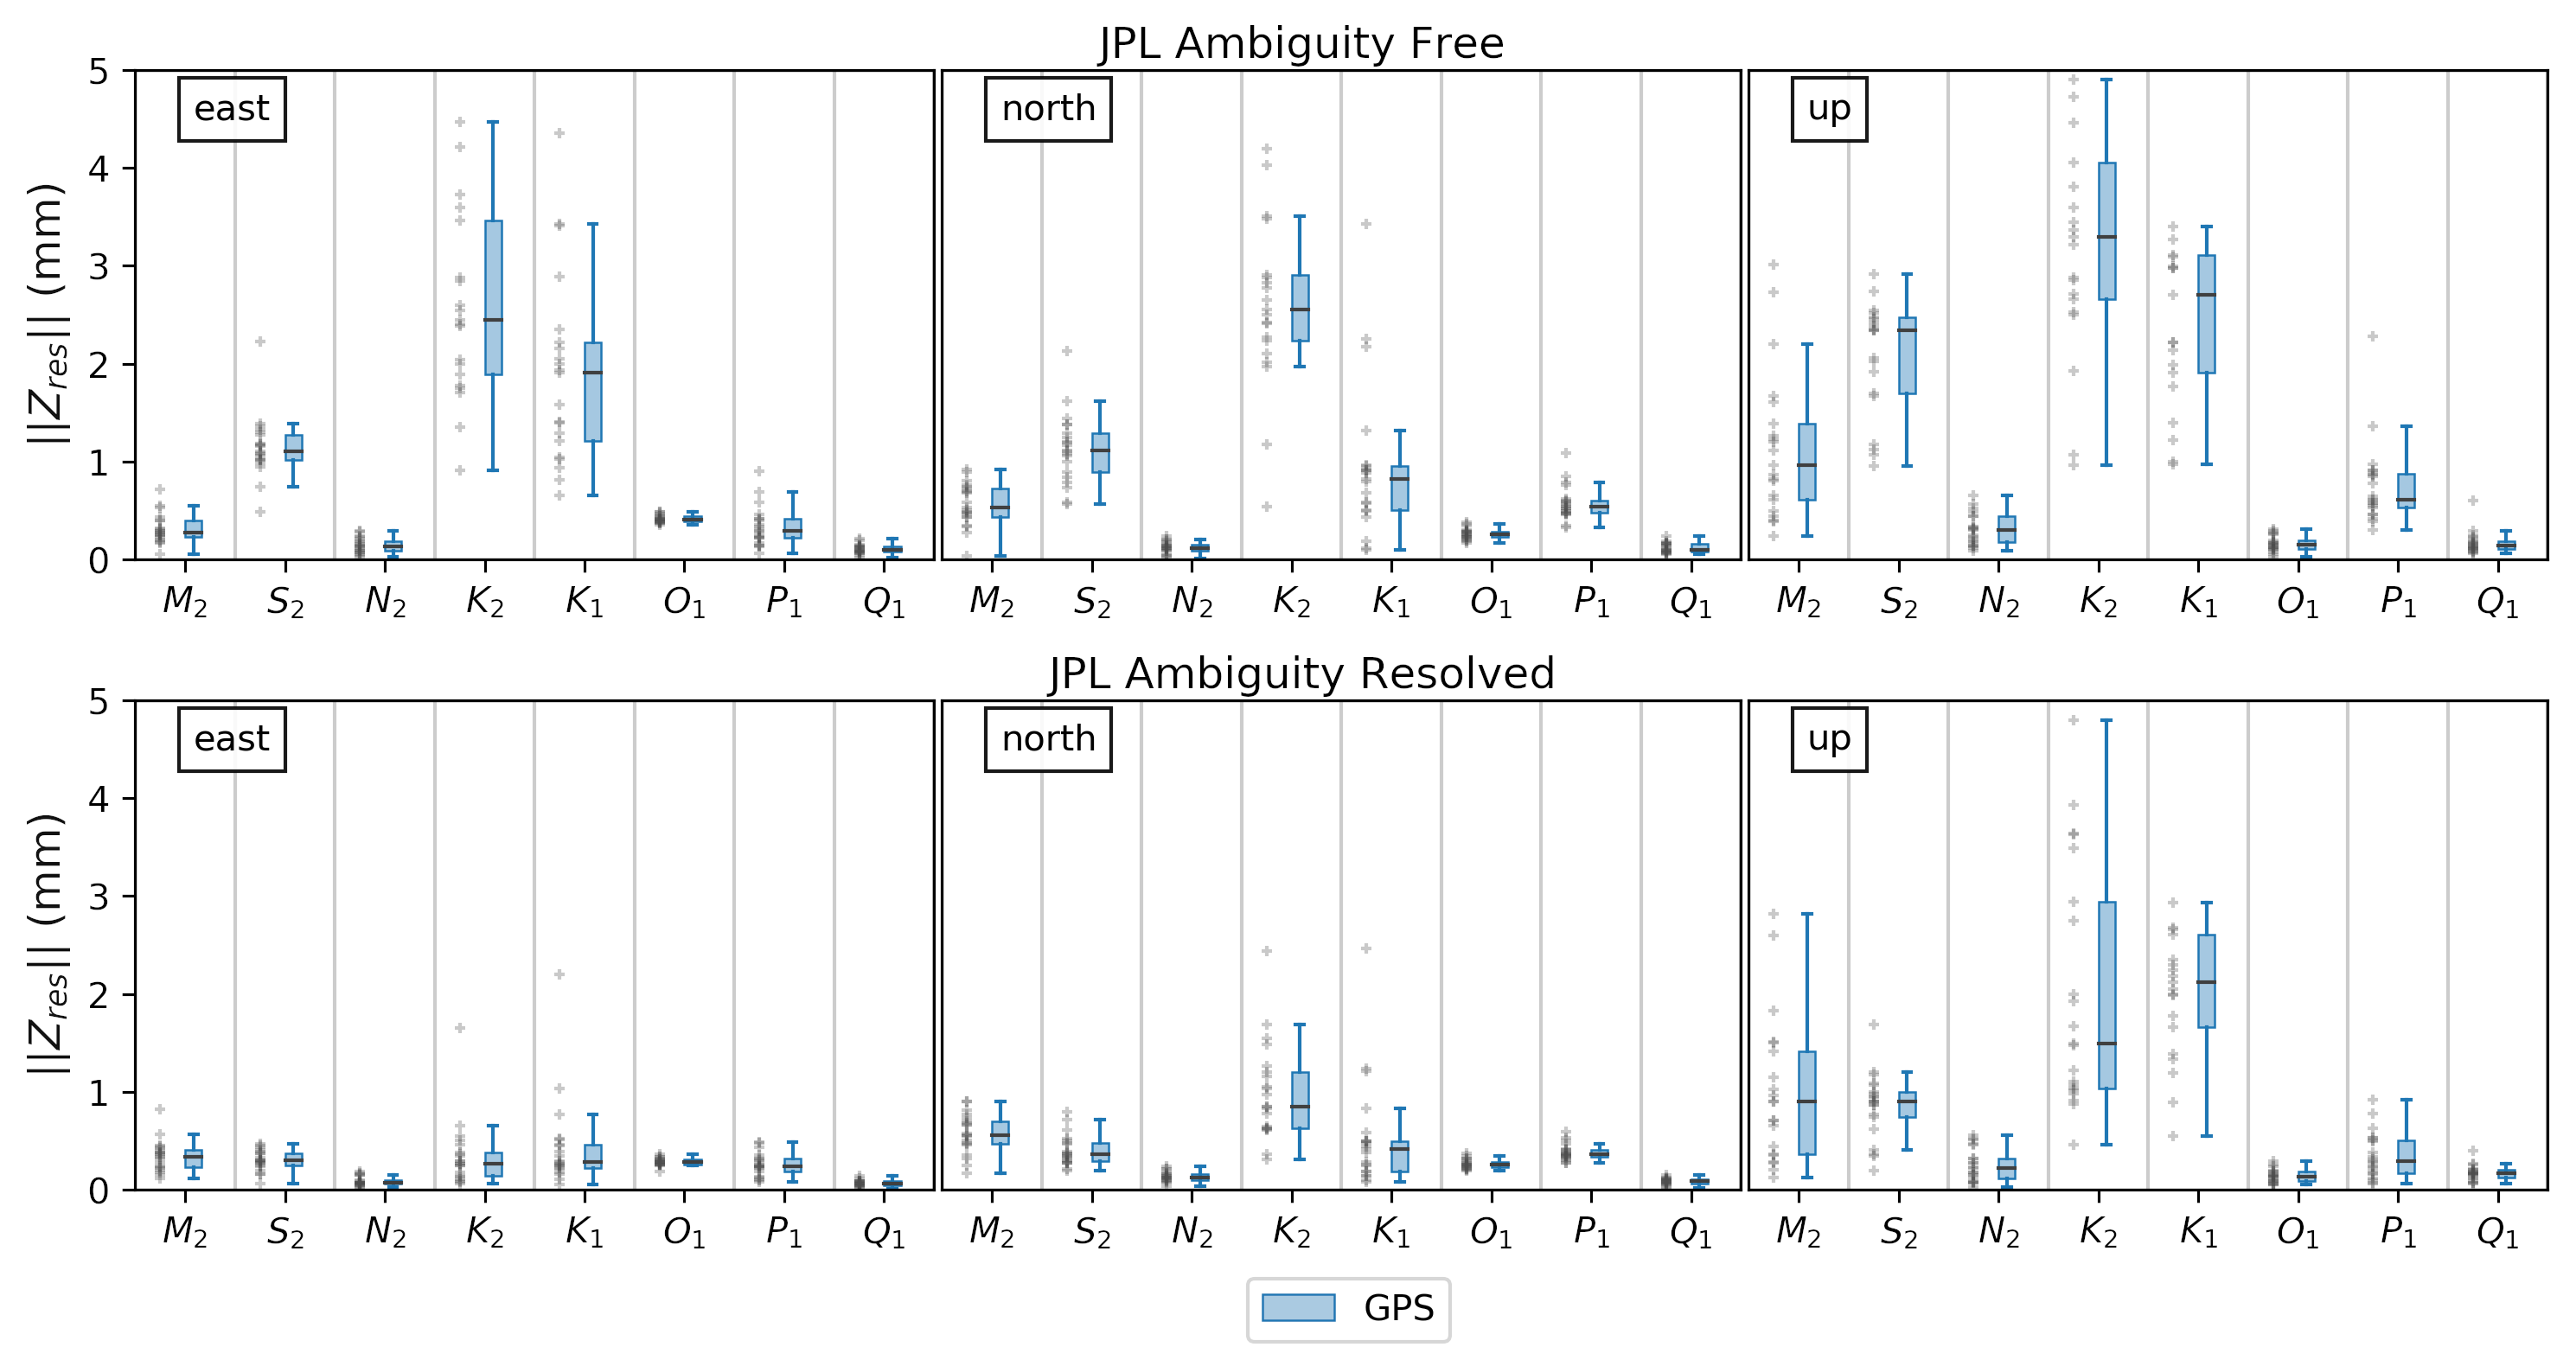
\includegraphics[width=17cm]{fig09.png}
\caption{Comparison of residual constituents’ estimates from GPS (top) and GPS AR (bottom) JPL native solutions. Grey crosses are as per Figure 3. As seen, most of constituents’ $\|Z_{res}\|$ distribution variances and medians are smaller while $S_2$ $\|Z_{res}\|$ bias is removed with AR solutions.}
\end{figure*}

Importantly, Figure 9 shows that enabling AR eliminates $\|Z_{res}\|$ bias in GPS and aligns the residual vectors with ESA/CODE GPS+GLONASS (Figure 3). Thus, the $S_2$ $\|Z_{res}\|$ bias was once again assessed with various elevation cutoff angles solutions. JPL GPS solutions, in the up component (Figure 10, left), show $S_2$ $\|Z_{res}\|$ bias to be constant between cutoff angles at about 1 mm with median $\|Z_{res}\|$ fluctuating around 3 mm. Similar behaviour was previously observed with solutions using ESA products (Fig.6).

%figure 10
\begin{figure}[t]
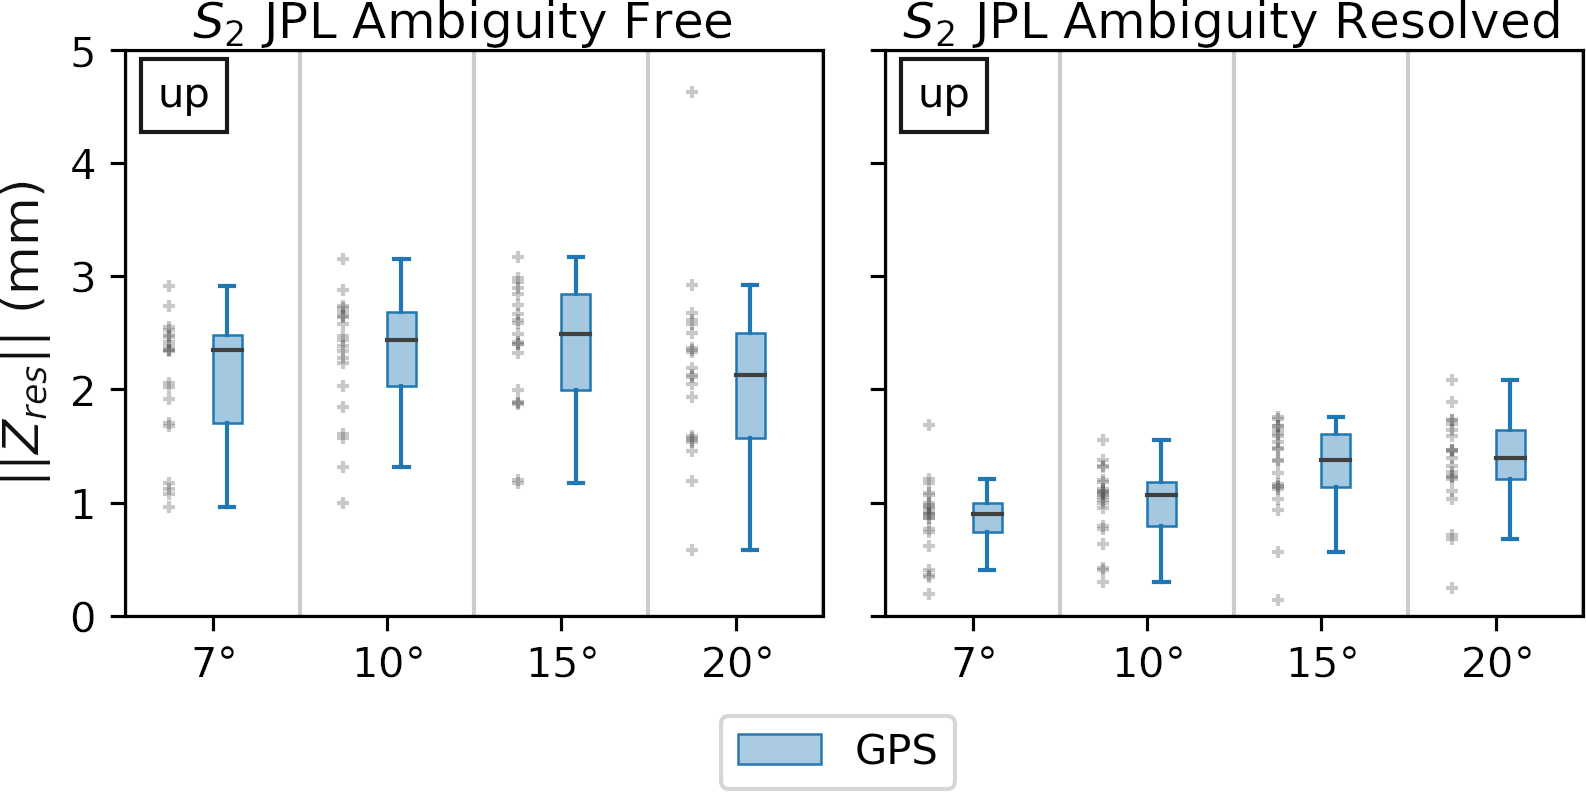
\includegraphics[width=8.3cm]{fig10.png}
\caption{GPS $S_2$ up constituent’s $\|Z_{res}\|$ change with elevation cutoff angle computed with JPL products floating AR (left) and integer AR (right). Grey crosses are as per Figure 3. As seen, AR helps in removing the bias and  decreases the $\|Z_{res}\|$ distribution variance.}
\end{figure}

Enabling integer ambiguity resolution (GPS AR) removes the $\sim$1 mm $S_2$ $\|Z_{res}\|$ bias completely at 7° and 10° elevation cutoff angles while leaving $\sim$ 0.4 mm bias at 15° and 20° in the up component. Consequently, up $\|Z_{res}\|$ medians change by 1-2 mm depending on elevation cutoff angle. Based on this observation, we expect that resolving ambiguities within PPP might help in solving, or at least minimising, the $S_2$ $\|Z_{res}\|$ present in ESA GPS and CODE GLONASS solutions. Eliminating biases in GPS and GLONASS separately should increase the stability and consistency of GPS+GLONASS $S_2$ $\|Z_{res}\|$.

\subsection{Impact of timeseries length}
\cite{Yuan2013} used a filter based harmonic parameter estimation approach and demonstrated the dependence of Kalman filter convergence and timeseries length for each of the eight major constituents. \cite{Yuan2013} concluded that after 1000 daily solutions convergence (minimized $\|Z_{res}\|$) was reached for lunar-only constituents ($M_2$, $N_2$, $O_1$, $Q_1$) while reporting solar-related constituents ($S_2$, $K_2$, $K_1$, $P_1$) were not fully converged even after 3000 daily solutions.

We assessed how $\|Z_{res}\|$ of each of 8 major constituents vary as a function of the time series length with kinematic estimation approach. The duration of the series varied by integer years and, to enable a complete analysis, we expanded the candidate solutions to 2019.0 and processed additional data with operational products: JPL repro3.0, ESA operational, CODE MGEX (CODE operational lack GLONASS clock corrections). While the goal of reprocessing campaign is to preserve consistency with operational products \citep{Griffiths2019}, based on previous results, we assumed that changing satellite orbit and clock products may produce substantial differences in problematic solar-related constituents ($S_2$, $K_2$, $K_1$, $P_1$). Thus, we first performed a comparison of ESA repro2 solutions (2010.0-2014.0) with the ESA operational product (2014.0-2019.0) which confirmed the hypothesis (Figure 11). GLONASS $\|\Delta Z_{res}\|$ show the smallest variance for $K_1$ and $K_2$ compared with GPS and GPS+GLONASS but are significant, up specifically, which might be related to the changes in GLONASS products processing. Considering $S_2$, the very same form of bias remains as previously seen with 2010.0-2014.0 dataset. This suggests symmetric deviation of repro2 and operational products solutions from the modelled value. The same explanation can be applied to the GPS-only $P_1$ up 0.5 mm $\|\Delta Z_{res}\|$ bias.

The results shown in Figure 12 are a composition of reprocessed products and operational products (years 5 to 9). We focus on $S_2$ up and $K_1$ up, as the most problematic diurnal constituents. The results align with general conclusions of \cite{Yuan2013} suggesting a weak relationship between timeseries length and $\|Z_{res}\|$ for solar-related constituents. However, if constituents selected according to optimum constellation strategy, $\|Z_{res}\|$ appear (see Fig. S4) stable over time, which suggests that even if there are changes in the products, they are not having an impact with this methodology.

%figure 11
\begin{figure*}[t]
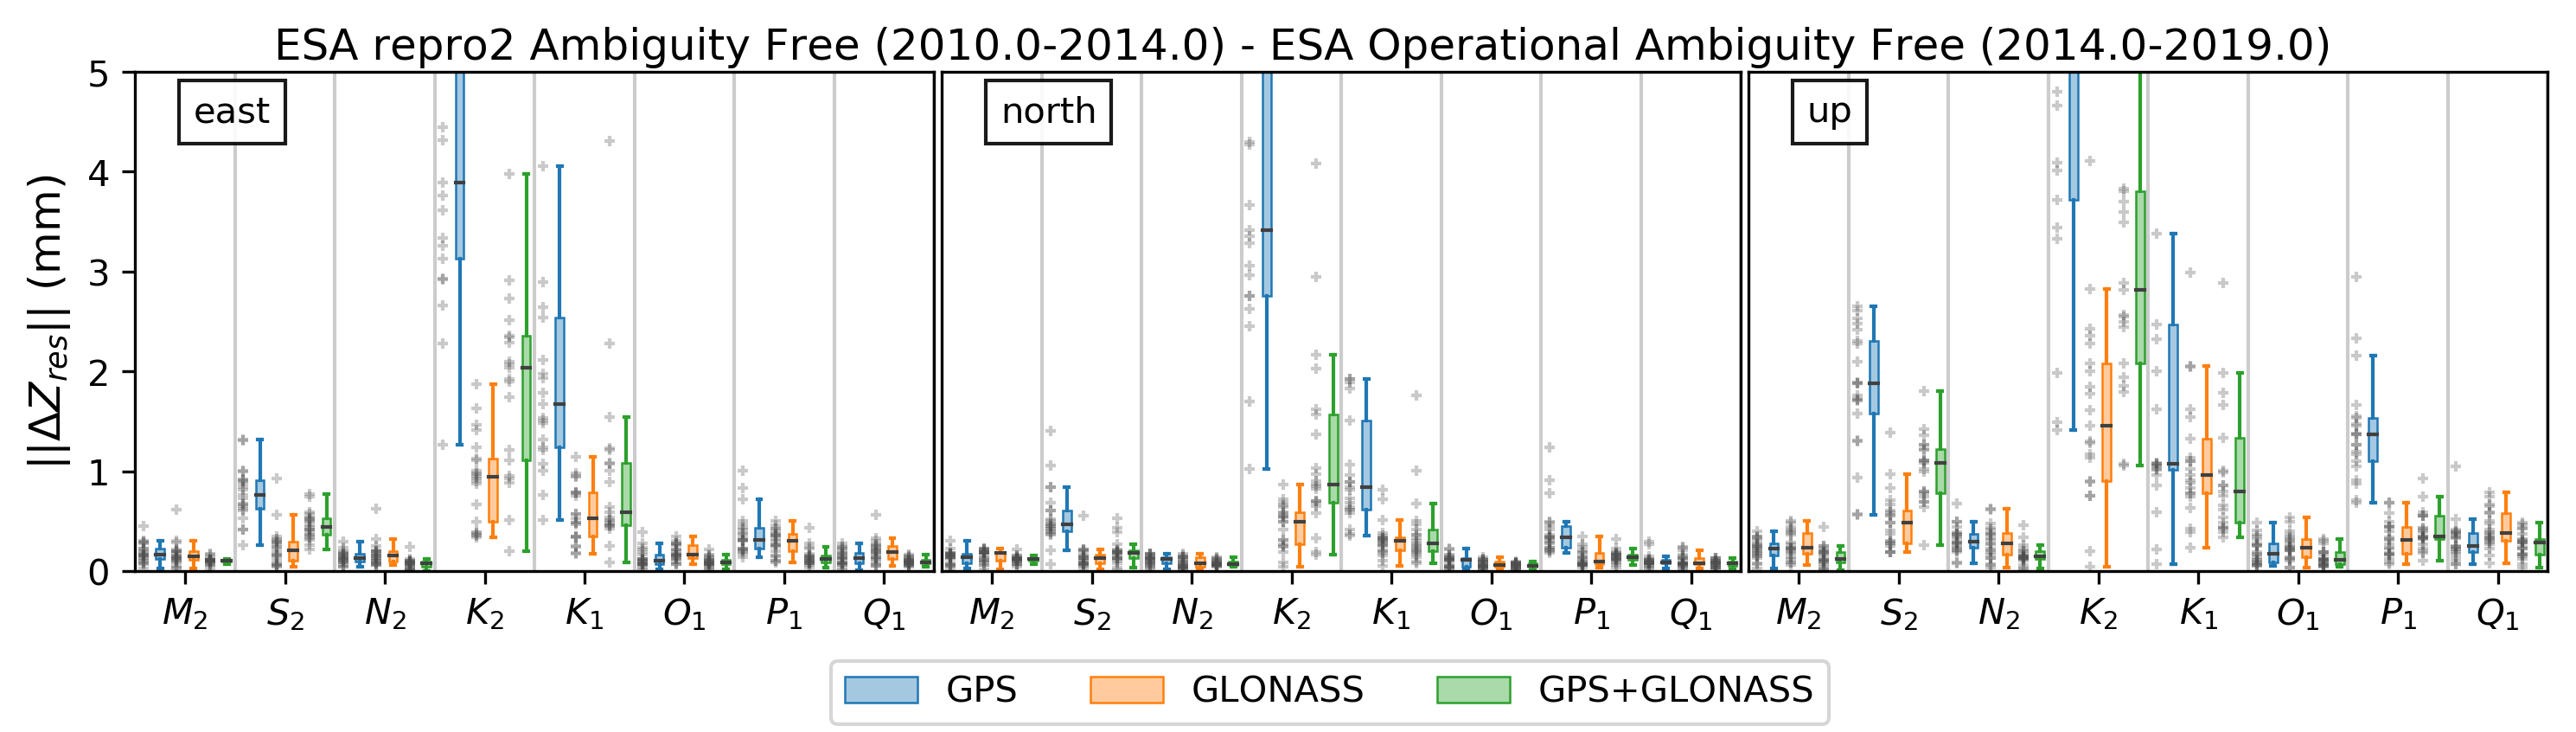
\includegraphics[width=17cm]{fig12.png}
\caption{OTL vector differences between ESA repro2 (2010.0-2014.0) and ESA operational (2014.0-2019.0) OTL estimates: GPS (blue), GLONASS (orange), GPS+GLONASS (green) constellation modes present. Grey crosses are as per Figure 3.}
\end{figure*}



%figure 12
\begin{figure*}[t]
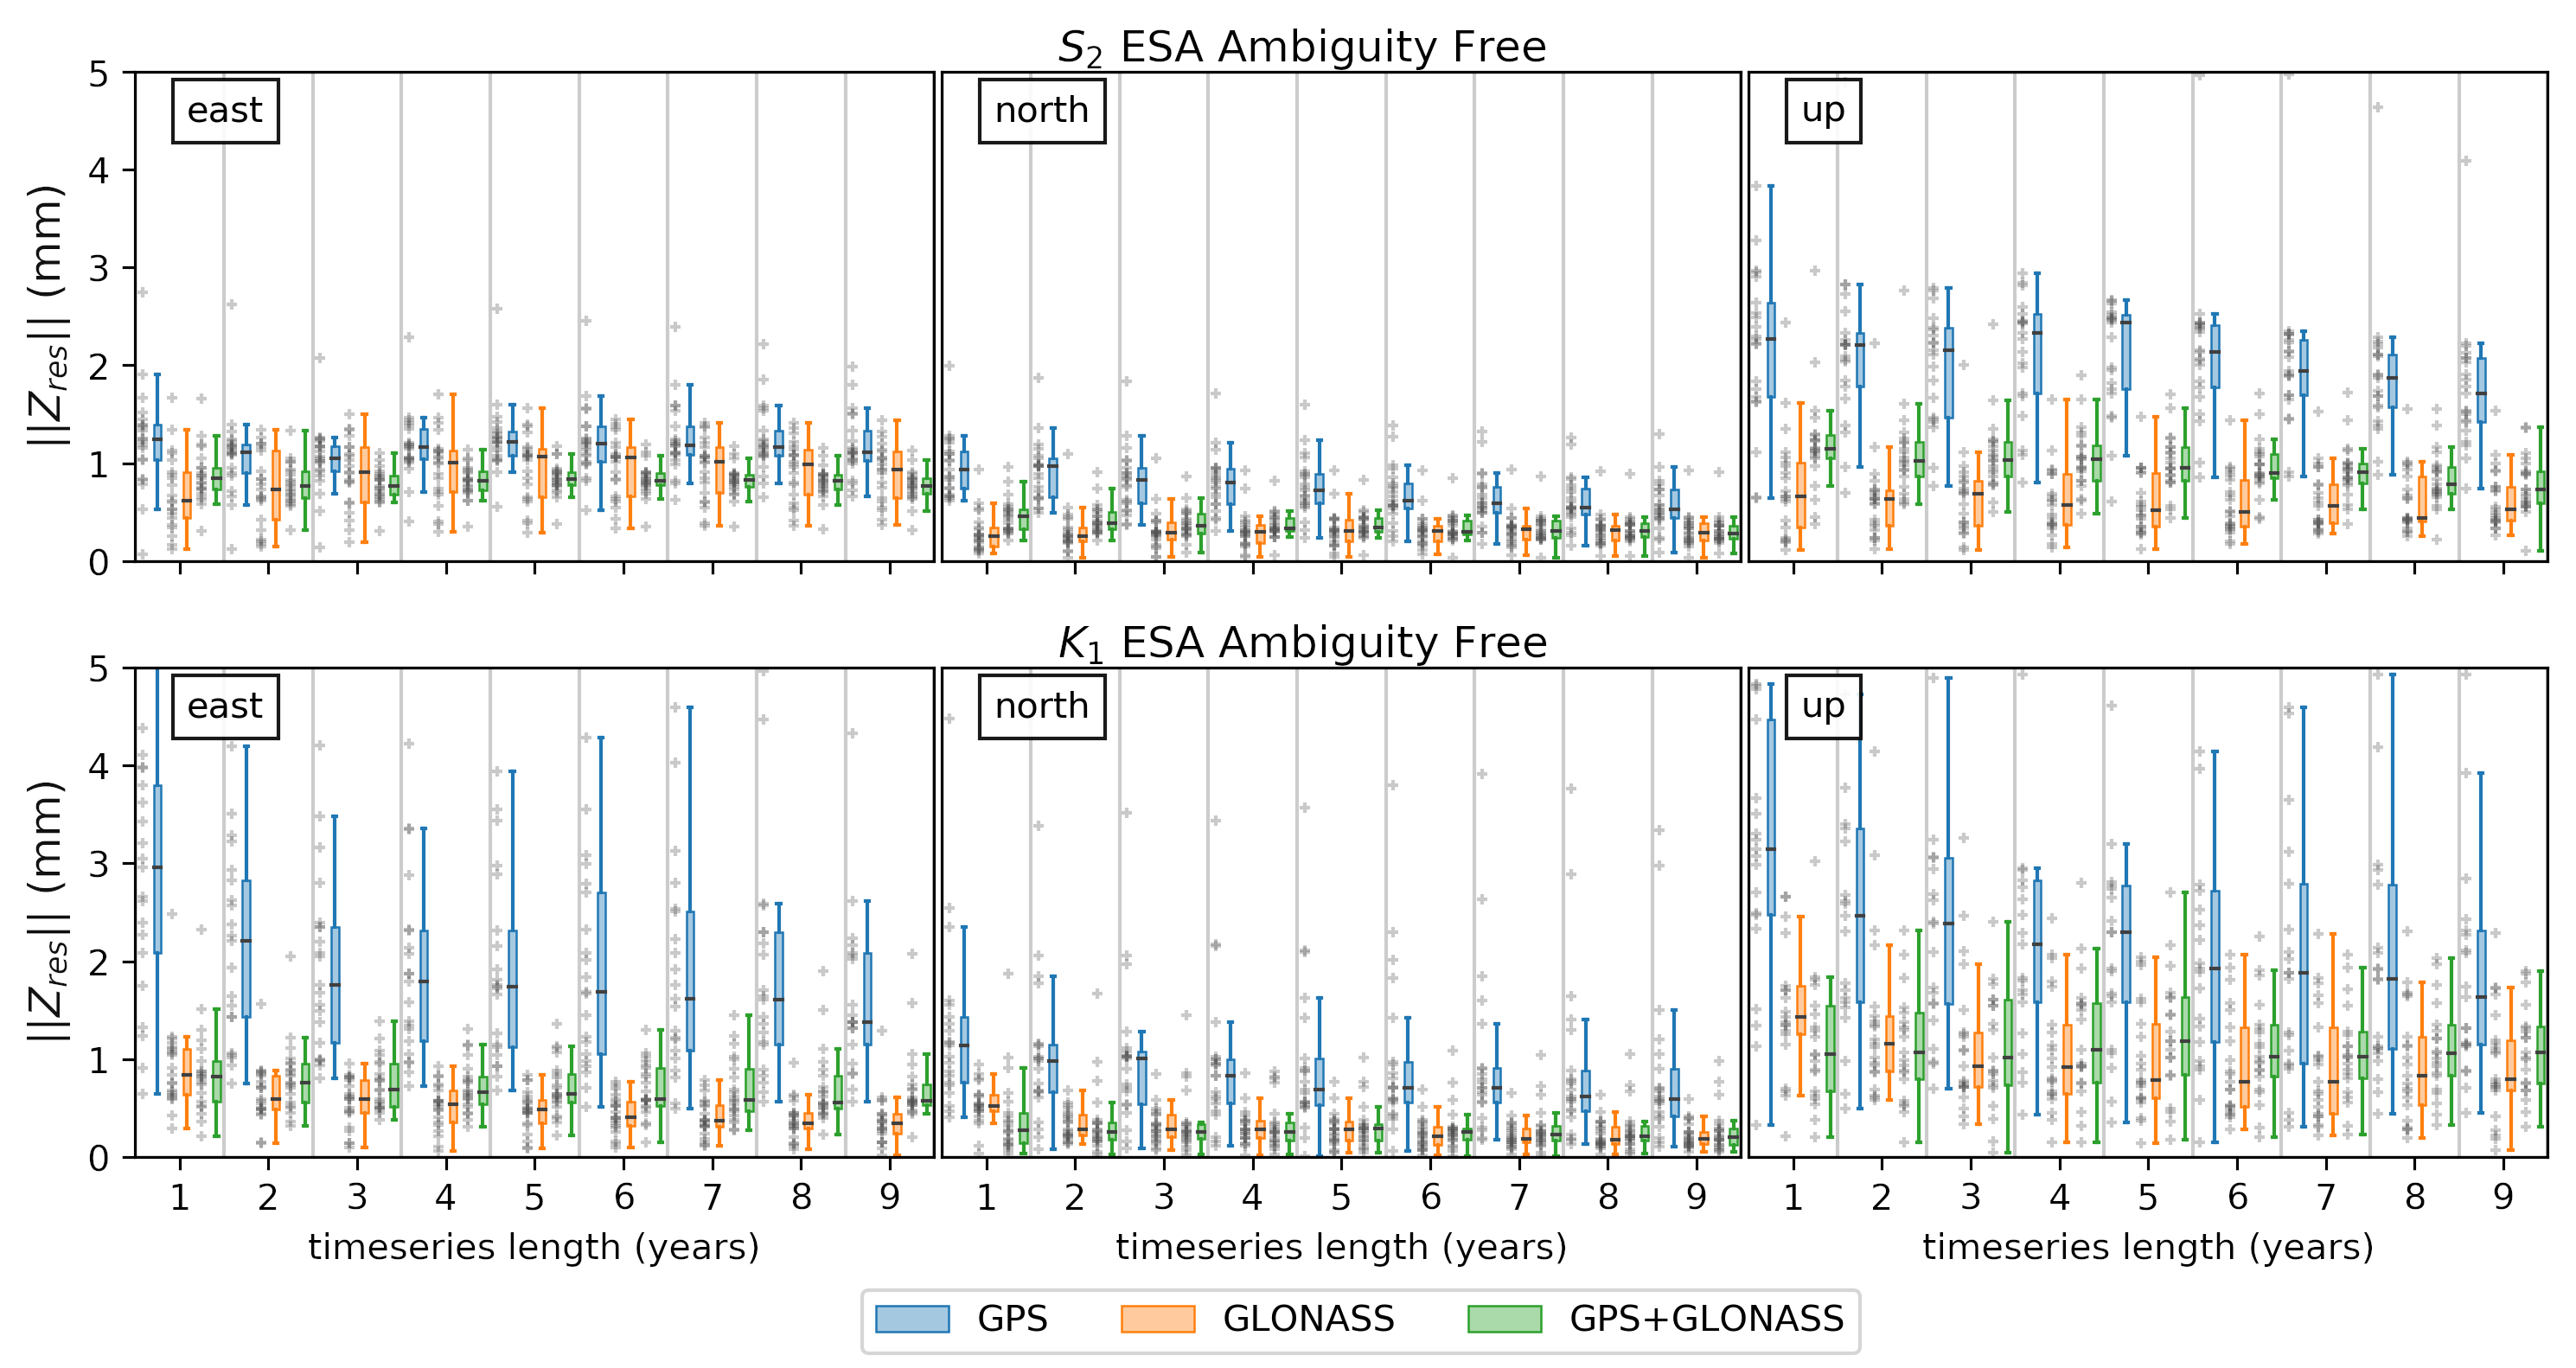
\includegraphics[width=17cm]{fig11.png}
\caption{Dependency of estimated $\|Z_{res}\|$ and timeseries’ length in years for two solar related constituents: $S_2$ (top), $K_1$ (bottom). GPS, GLONASS and GPS+GLONASS PPP solutions in blue, orange and green, respectively using ESA products. Grey crosses are as per Figure 3. Note that 1 to 4 years of timeseries length use ESA repro2 while the rest uses a combination of ESA repro2 and ESA operational products.}
\end{figure*}

\conclusions %% \conclusions[modified heading if necessary]
We expand the GPS-only methodology of ocean tide loading displacement estimation described in \cite{Penna2015} with GLONASS constellation and assess the performance of GPS and GLONASS for estimation of eight major ocean tide loading constituents in stand-alone modes and in a combined GPS+GLONASS mode. We examine data from 21 sites from the UK and western Europe over a period of 2010.0-2014.0 through processing data in kinematic PPP using products from three different analysis centres: CODE, ESA and JPL. The latter was also used to assess the effect of GPS ambiguity fixing on estimated ocean tide loading displacement. All solutions were intercompared to gain an insight into the sensitivities of the constituent estimates to different choices of satellite orbit and clock products and constellation configurations.

We find that no single constellation mode solution for all eight major tidal constituents exists. However, we do find that GLONASS-based estimates show a comparable level of performance to ambiguity-free GPS for $M_2$, $N_2$, $O_1$, $P_1$ and $Q_1$ while showing improved results for $K_2$ and $K_1$. Alternatively, this optimal solution can be constructed from the combination of constellation modes for each constituent and component for the case of GPS and GLONASS presence.

We show that ambiguity-free GPS+GLONASS solutions show a similar level of precision as GPS with ambiguities resolved (GPS AR), with $P_1$ estimates using GPS+GLONASS showing improved precision and stability. The $K_2$ and $K_1$ constituents, which are known to be problematic in GPS solutions, are still unusable in GPS+GLONASS solutions, due to propagation of GPS related errors. The $S_2$ constituent also cannot be reliably recovered with GPS+GLONASS as GLONASS shows dependency between the estimates and chosen elevation cutoff angle. GPS-based estimates of $S_2$ show a constant bias when ambiguity resolution is not implemented, but this is removed by resolving the ambiguities to integers. GLONASS-based estimates show a comparable level of performance to ambiguity-free GPS for $M_2$, $N_2$, $O_1$, $P_1$ and $Q_1$ while showing improved results for $K_2$ and $K_1$.

Additional comparison of OTL estimates from reprocessed and operational products shows that GLONASS estimates of $K_2$ and $K_1$ show differences in the up and, to the lesser extent in the east, components when using different products.

Considering the above, we suggest that estimation of $K_1$ and $K_2$ constituents is best undertaken using GLONASS only solutions with an emphasis towards the north component where it is most stable. $M_2$, $S_2$, $N_2$, $O_1$ and $Q_1$ can be reliably estimated from combined GPS+GLONASS or GPS AR solutions while $P_1$ is best with GPS+GLONASS.

Integer ambiguity resolution was not possible in the GLONASS or GPS+GLONASS solutions tested here due to limitations in the products available. However, evidence from our GPS AR testing suggests that further increases in precision and stability will be seen when AR fixing can be performed which should have a positive impact on solar-related constituents.


%% The following commands are for the statements about the availability of data sets and/or software code corresponding to the manuscript.
%% It is strongly recommended to make use of these sections in case data sets and/or software code have been part of your research the article is based on.

% \codeavailability{} %% use this section when having only software code available

% \dataavailability{} %% use this section when having only data sets available


\codedataavailability{GNSS data were obtained from the Natural Environment Research Council (NERC) British Isles continuous GNSS Facility (BIGF), www.bigf.ac.uk and the International GNSS Service (IGS), www.igs.org. OTL values and TPXO.7.2 OTL grid were obtained from free ocean tide loading provider, holt.oso.chalmers.se/loading/. CODE REPRO\_2015 and CODE MGEX orbit and clock products were obtained from the University of Bern, ftp.aiub.unibe.ch/REPRO\_2015/ and ftp.aiub.unibe.ch/CODE\_MGEX/ respectively, ESA repro2 and operational from the Crustal Dynamics Data Information System (CDDIS), JPL repro 2.1 and repro 3.0 from NASA Jet Propulsion Laboratory, sideshow.jpl.nasa.gov/pub/.

GipsyX binaries were provided under license from JPL. Eterna tidal analysis and prediction software with source code was acquired from International Geodynamics and Earth Tide Service (IGETS), igets.u-strasbg.fr/soft\_and\_tool.php.
The source code of GipsyX wrapper developed to facilitate the processing, analyse output and undertake plotting can be found at: github.com/bmatv/GipsyX\_Wrapper.} %% use this section when having data sets and software code available


% \sampleavailability{TEXT} %% use this section when having geoscientific samples available


% \videosupplement{TEXT} %% use this section when having video supplements available


% \appendix
% \section{} %% Appendix A

% \subsection{} %% Appendix A1, A2, etc.


% \noappendix %% use this to mark the end of the appendix section. Otherwise the figures might be numbered incorrectly (e.g. 10 instead of 1).

%% Regarding figures and tables in appendices, the following two options are possible depending on your general handling of figures and tables in the manuscript environment:

%% Option 1: If you sorted all figures and tables into the sections of the text, please also sort the appendix figures and appendix tables into the respective appendix sections.
%% They will be correctly named automatically.

%% Option 2: If you put all figures after the reference list, please insert appendix tables and figures after the normal tables and figures.
%% To rename them correctly to A1, A2, etc., please add the following commands in front of them:

% \appendixfigures %% needs to be added in front of appendix figures

% \appendixtables %% needs to be added in front of appendix tables

%% Please add \clearpage between each table and/or figure. Further guidelines on figures and tables can be found below.

\authorcontribution{BM facilitated processing of the GNSS data with GipsyX and analysis of the resulting timeseries under the supervision of MK and CW. All authors contributed to the discussion of the results and writing of the manuscript.} %% this section is mandatory

\competinginterests{The authors declare that they have no conflicts of interest.} %% this section is mandatory even if you declare that no competing interests are present

% \disclaimer{TEXT} %% optional section

\begin{acknowledgements}
The services of the Natural Environment Research Council (NERC) British Isles continuous GNSS Facility (BIGF), www.bigf.ac.uk, in providing archived GNSS data to this study, are gratefully acknowledged. We are grateful to NASA Jet Propulsion Laboratory for the GipsyX software, products and support. We thank IGS, www.igs.org, for providing GNSS data and ESA reprocessed products; CODE, www.aiub.unibe.ch, for providing reprocessed products. We thank Klaus Schueller for advice and discussion on Eterna software. The services of TPAC High Performance Computing Facility are acknowledged gratefully. We gratefully acknowledge Machiel Bos whose support and discussion were vital for the project. We thank the Free Ocean Loading Provider for the OTL computation services and for providing the OTL grid that was used in Figure 1.
\end{acknowledgements}




%% REFERENCES

%% The reference list is compiled as follows:

% \begin{thebibliography}{}

% \bibitem[AUTHOR(YEAR)]{LABEL1}
% REFERENCE 1

% \bibitem[AUTHOR(YEAR)]{LABEL2}
% REFERENCE 2

% \end{thebibliography}

%% Since the Copernicus LaTeX package includes the BibTeX style file copernicus.bst,
%% authors experienced with BibTeX only have to include the following two lines:
%%
\bibliographystyle{copernicus}
\bibliography{references.bib}
%%
%% URLs and DOIs can be entered in your BibTeX file as:
%%
%% URL = {http://www.xyz.org/~jones/idx_g.htm}
%% DOI = {10.5194/xyz}


%% LITERATURE CITATIONS
%%
%% command & example result
%% \citet{jones90}| & Jones et al. (1990)
%% \citep{jones90}| & (Jones et al., 1990)
%% \citep{jones90,jones93}| & (Jones et al., 1990, 1993)
%% \citep[p.~32]{jones90}| & (Jones et al., 1990, p.~32)
%% \citep[e.g.,][]{jones90}| & (e.g., Jones et al., 1990)
%% \citep[e.g.,][p.~32]{jones90}| & (e.g., Jones et al., 1990, p.~32)
%% \citeauthor{jones90}| & Jones et al.
%% \citeyear{jones90}| & 1990



%% FIGURES

%% When figures and tables are placed at the end of the MS (article in one-column style), please add \clearpage
%% between bibliography and first table and/or figure as well as between each table and/or figure.


%% ONE-COLUMN FIGURES

%%f
%\begin{figure}[t]
%\includegraphics[width=8.3cm]{FILE NAME}
%\caption{TEXT}
%\end{figure}
%
%%% TWO-COLUMN FIGURES
%
%%f
%\begin{figure*}[t]
%\includegraphics[width=12cm]{FILE NAME}
%\caption{TEXT}
%\end{figure*}
%
%
%%% TABLES
%%%
%%% The different columns must be seperated with a & command and should
%%% end with \\ to identify the column brake.
%
%%% ONE-COLUMN TABLE
%
%%t
%\begin{table}[t]
%\caption{TEXT}
%\begin{tabular}{column = lcr}
%\tophline
%
%\middlehline
%
%\bottomhline
%\end{tabular}
%\belowtable{} % Table Footnotes
%\end{table}
%
%%% TWO-COLUMN TABLE
%
%%t
%\begin{table*}[t]
%\caption{TEXT}
%\begin{tabular}{column = lcr}
%\tophline
%
%\middlehline
%
%\bottomhline
%\end{tabular}
%\belowtable{} % Table Footnotes
%\end{table*}
%
%%% LANDSCAPE TABLE
%
%%t
%\begin{sidewaystable*}[t]
%\caption{TEXT}
%\begin{tabular}{column = lcr}
%\tophline
%
%\middlehline
%
%\bottomhline
%\end{tabular}
%\belowtable{} % Table Footnotes
%\end{sidewaystable*}
%
%
%%% MATHEMATICAL EXPRESSIONS
%
%%% All papers typeset by Copernicus Publications follow the math typesetting regulations
%%% given by the IUPAC Green Book (IUPAC: Quantities, Units and Symbols in Physical Chemistry,
%%% 2nd Edn., Blackwell Science, available at: http://old.iupac.org/publications/books/gbook/green_book_2ed.pdf, 1993).
%%%
%%% Physical quantities/variables are typeset in italic font (t for time, T for Temperature)
%%% Indices which are not defined are typeset in italic font (x, y, z, a, b, c)
%%% Items/objects which are defined are typeset in roman font (Car A, Car B)
%%% Descriptions/specifications which are defined by itself are typeset in roman font (abs, rel, ref, tot, net, ice)
%%% Abbreviations from 2 letters are typeset in roman font (RH, LAI)
%%% Vectors are identified in bold italic font using \vec{x}
%%% Matrices are identified in bold roman font
%%% Multiplication signs are typeset using the LaTeX commands \times (for vector products, grids, and exponential notations) or \cdot
%%% The character * should not be applied as mutliplication sign
%
%
%%% EQUATIONS
%
%%% Single-row equation
%
%\begin{equation}
%
%\end{equation}
%
%%% Multiline equation
%
%\begin{align}
%& 3 + 5 = 8\\
%& 3 + 5 = 8\\
%& 3 + 5 = 8
%\end{align}
%
%
%%% MATRICES
%
%\begin{matrix}
%x & y & z\\
%x & y & z\\
%x & y & z\\
%\end{matrix}
%
%
%%% ALGORITHM
%
%\begin{algorithm}
%\caption{...}
%\label{a1}
%\begin{algorithmic}
%...
%\end{algorithmic}
%\end{algorithm}
%
%
%%% CHEMICAL FORMULAS AND REACTIONS
%
%%% For formulas embedded in the text, please use \chem{}
%
%%% The reaction environment creates labels including the letter R, i.e. (R1), (R2), etc.
%
%\begin{reaction}
%%% \rightarrow should be used for normal (one-way) chemical reactions
%%% \rightleftharpoons should be used for equilibria
%%% \leftrightarrow should be used for resonance structures
%\end{reaction}
%
%
%%% PHYSICAL UNITS
%%%
%%% Please use \unit{} and apply the exponential notation


\end{document}
